% !TeX spellcheck = de_DE
\documentclass[a4paper]{scrartcl}

\usepackage[utf8]{inputenc}
\usepackage[T1]{fontenc}
\usepackage{lmodern}
\usepackage[naustrian]{babel}
\usepackage{amsmath}
\usepackage{mathtools}
\usepackage{verbatim}
\usepackage{scrpage2}
\usepackage[dvipsnames]{xcolor}
\usepackage{titling}
\usepackage{a4wide}
\usepackage{pdfpages}
\usepackage{tikz}
\usepackage{titling}
\usepackage{float}


\pagestyle{scrheadings}
\clearscrheadfoot



%% scource-code listings
\usepackage{listingsutf8, scrhack}
\usepackage{courier}
\lstset{%
    basicstyle=\footnotesize\ttfamily,
    breaklines=true,
    commentstyle=\color{OliveGreen},
    keywordstyle=\color{MidnightBlue},
    stringstyle=\color{Maroon},
    escapeinside={\%*}{*)},
    inputencoding=utf8/latin1,
    frame=single,
    numbers=left,
    stepnumber=1
}

\begin{document}

\ofoot{\pagemark}

\tableofcontents
\newpage

\section{Mainboard}
\subsection{MCU}

Der Prozessor wurde hauptsächlich wegen seinem Reichtum an UART-Modulen ausgewählt. Wir benötigen hier drei Stück: GPS, Bluetooth und Debugging über UART-to-USB chip\\Außerdem haben wir bereits Erfahrung mit Cortex-M0-Prozessoren wie diesem im Unterricht gesammelt.\\Der Controller ist in einem LQFP64 Gehäuse verpackt, das ohne Probleme per Hand gelötet werden kann.

\begin{figure}[H]\centering
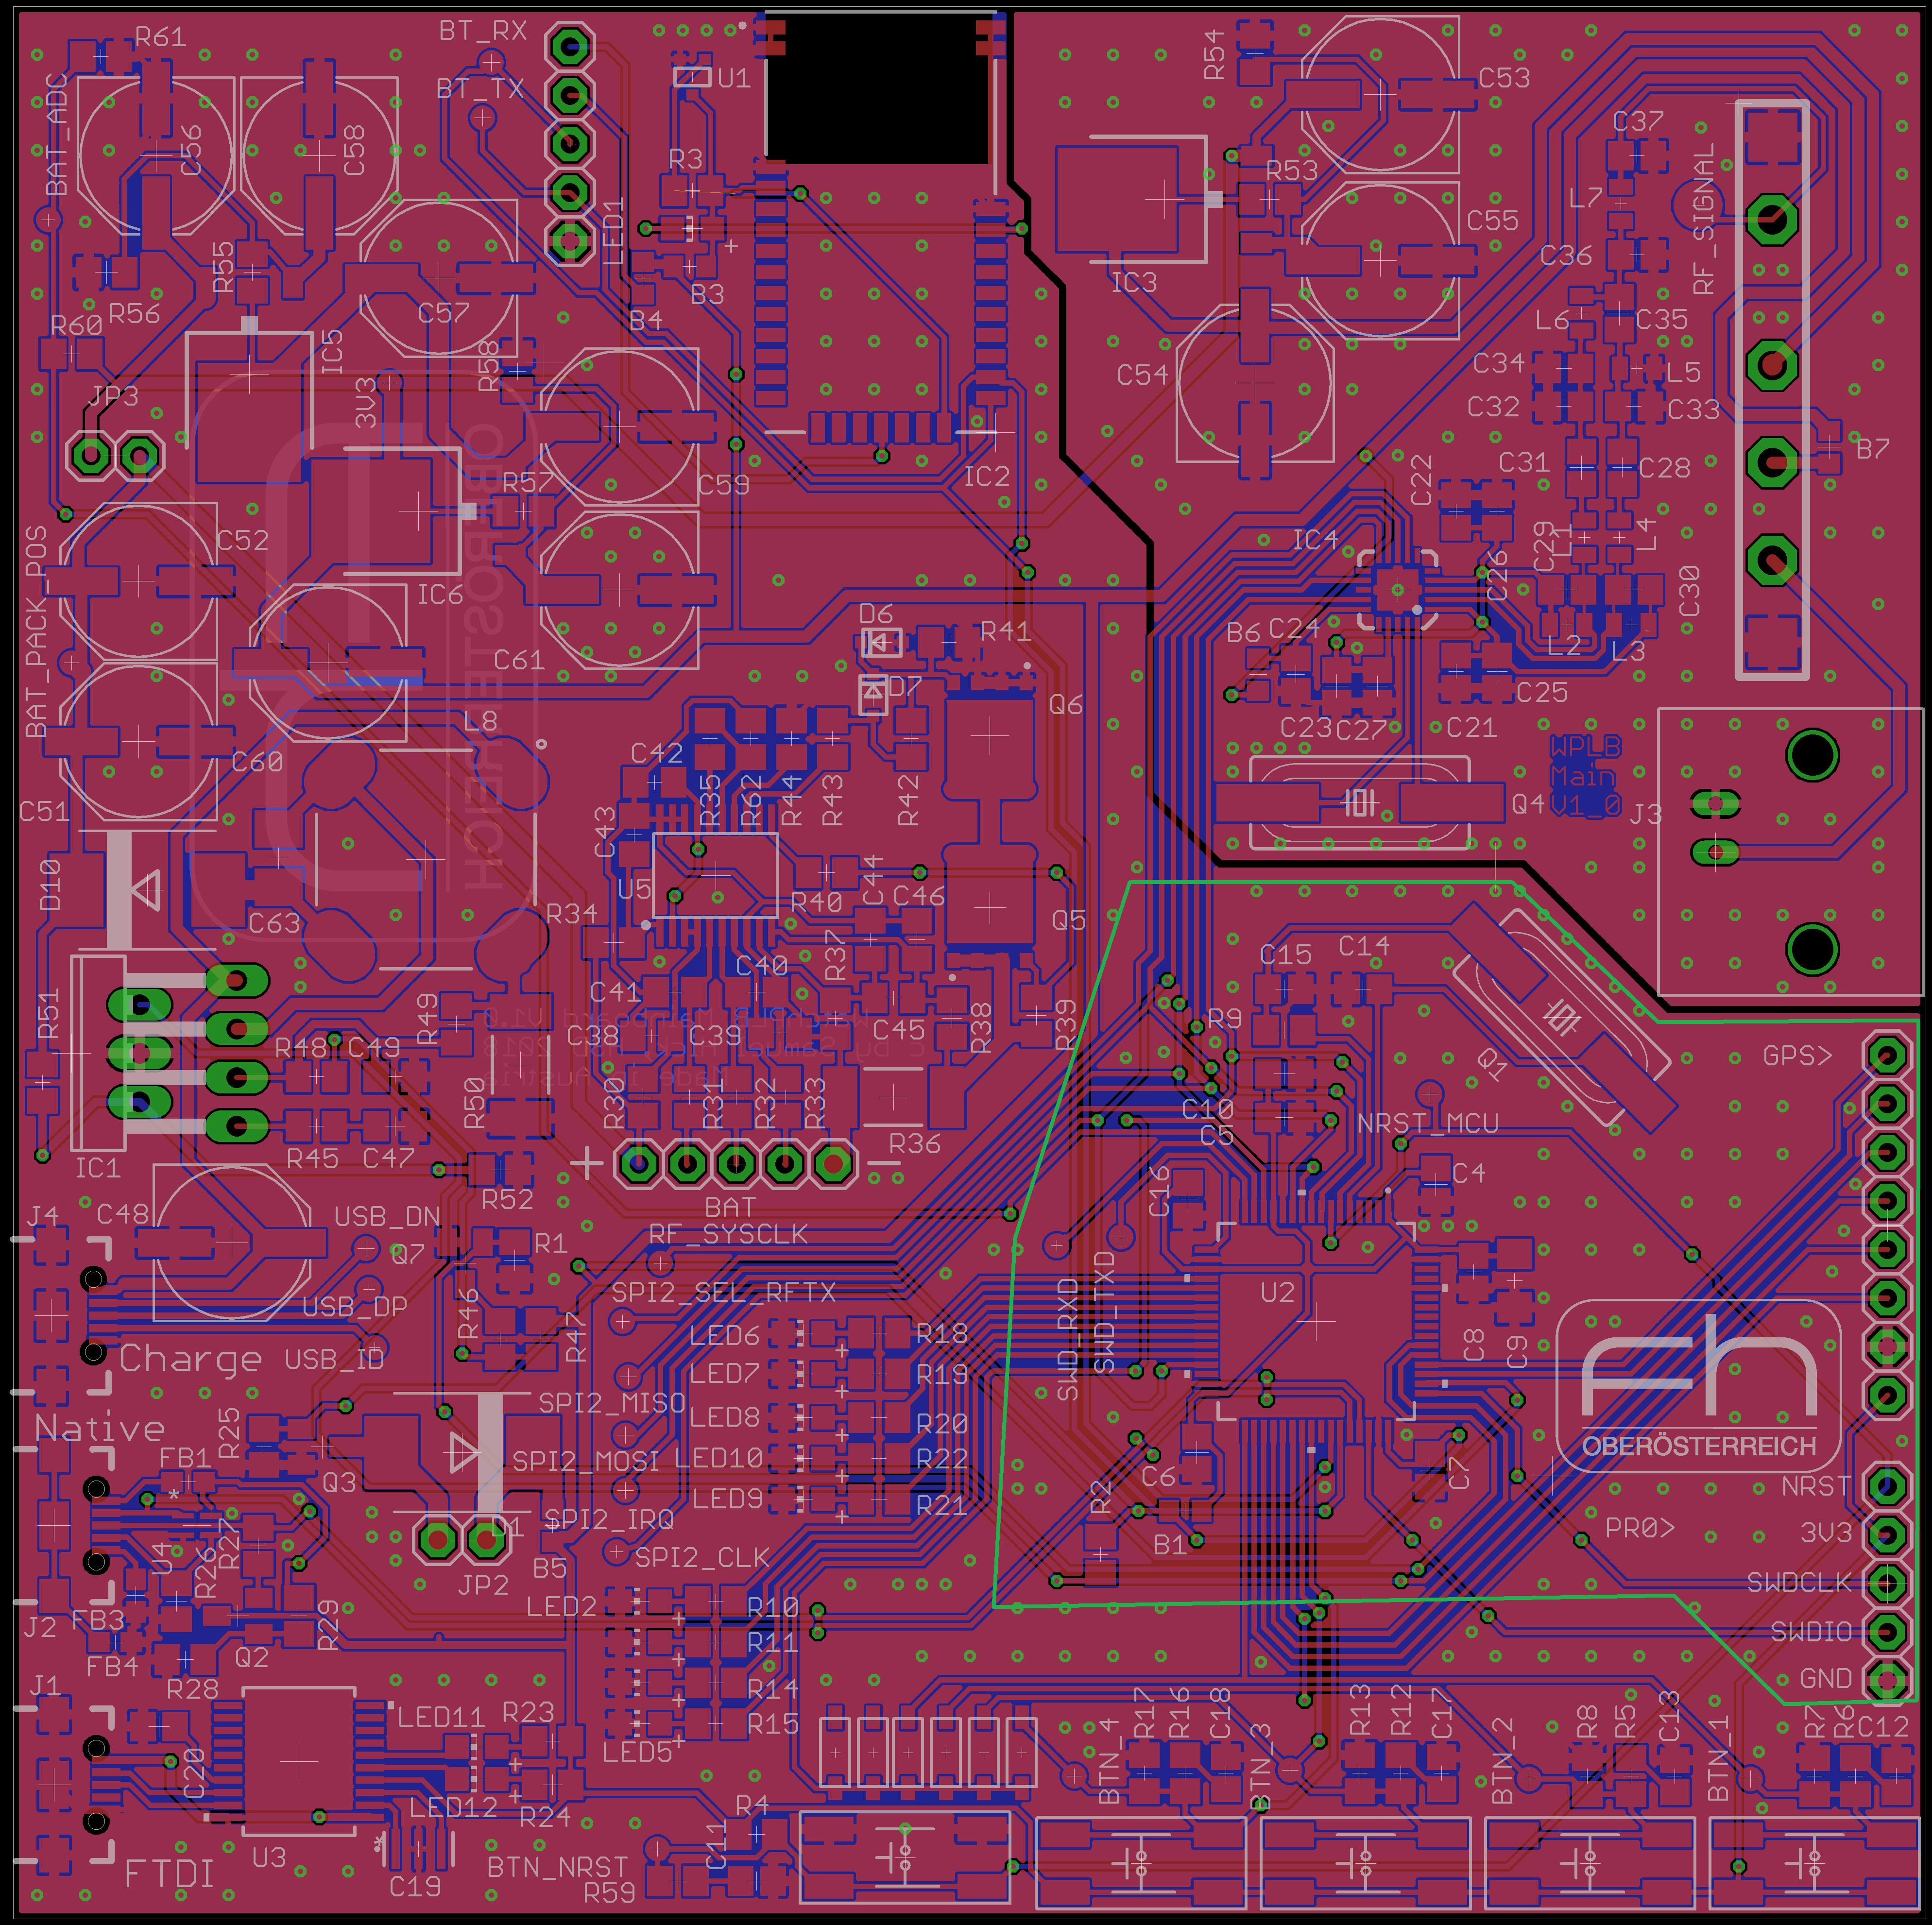
\includegraphics[page=1, angle=0, width=\linewidth]{../Documentation/pics/mainboard_mcu.png}
\caption{Hauptplatine, Baugruppe MCU grün umrahmt}
\end{figure}

\begin{figure}[H]\centering
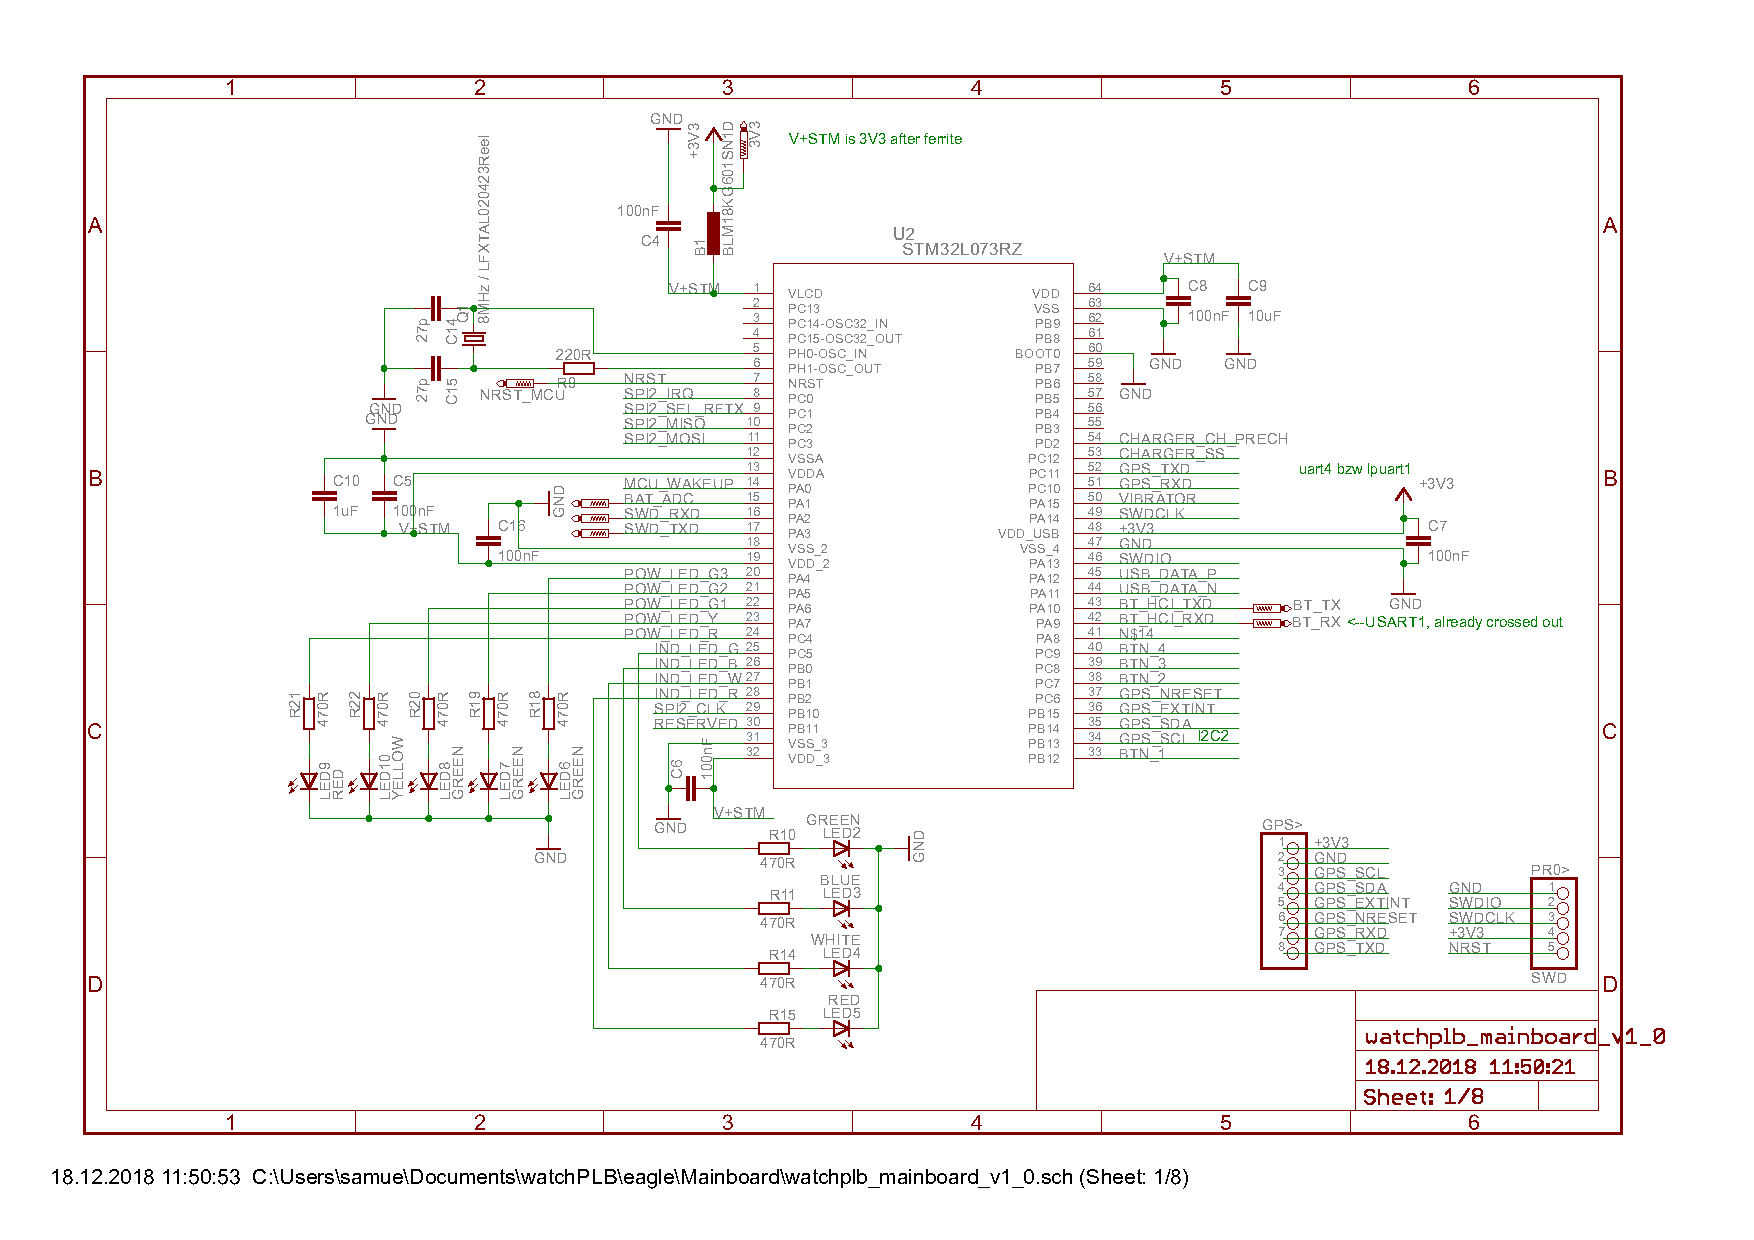
\includegraphics[page=1, angle=90, width=\linewidth]{../eagle/Mainboard/watchplb_mainboard_v1_0.pdf}
\caption{Schaltplanteil Mikrocontroller STM32L073RZ}
\end{figure}

\begin{figure}[H]\centering
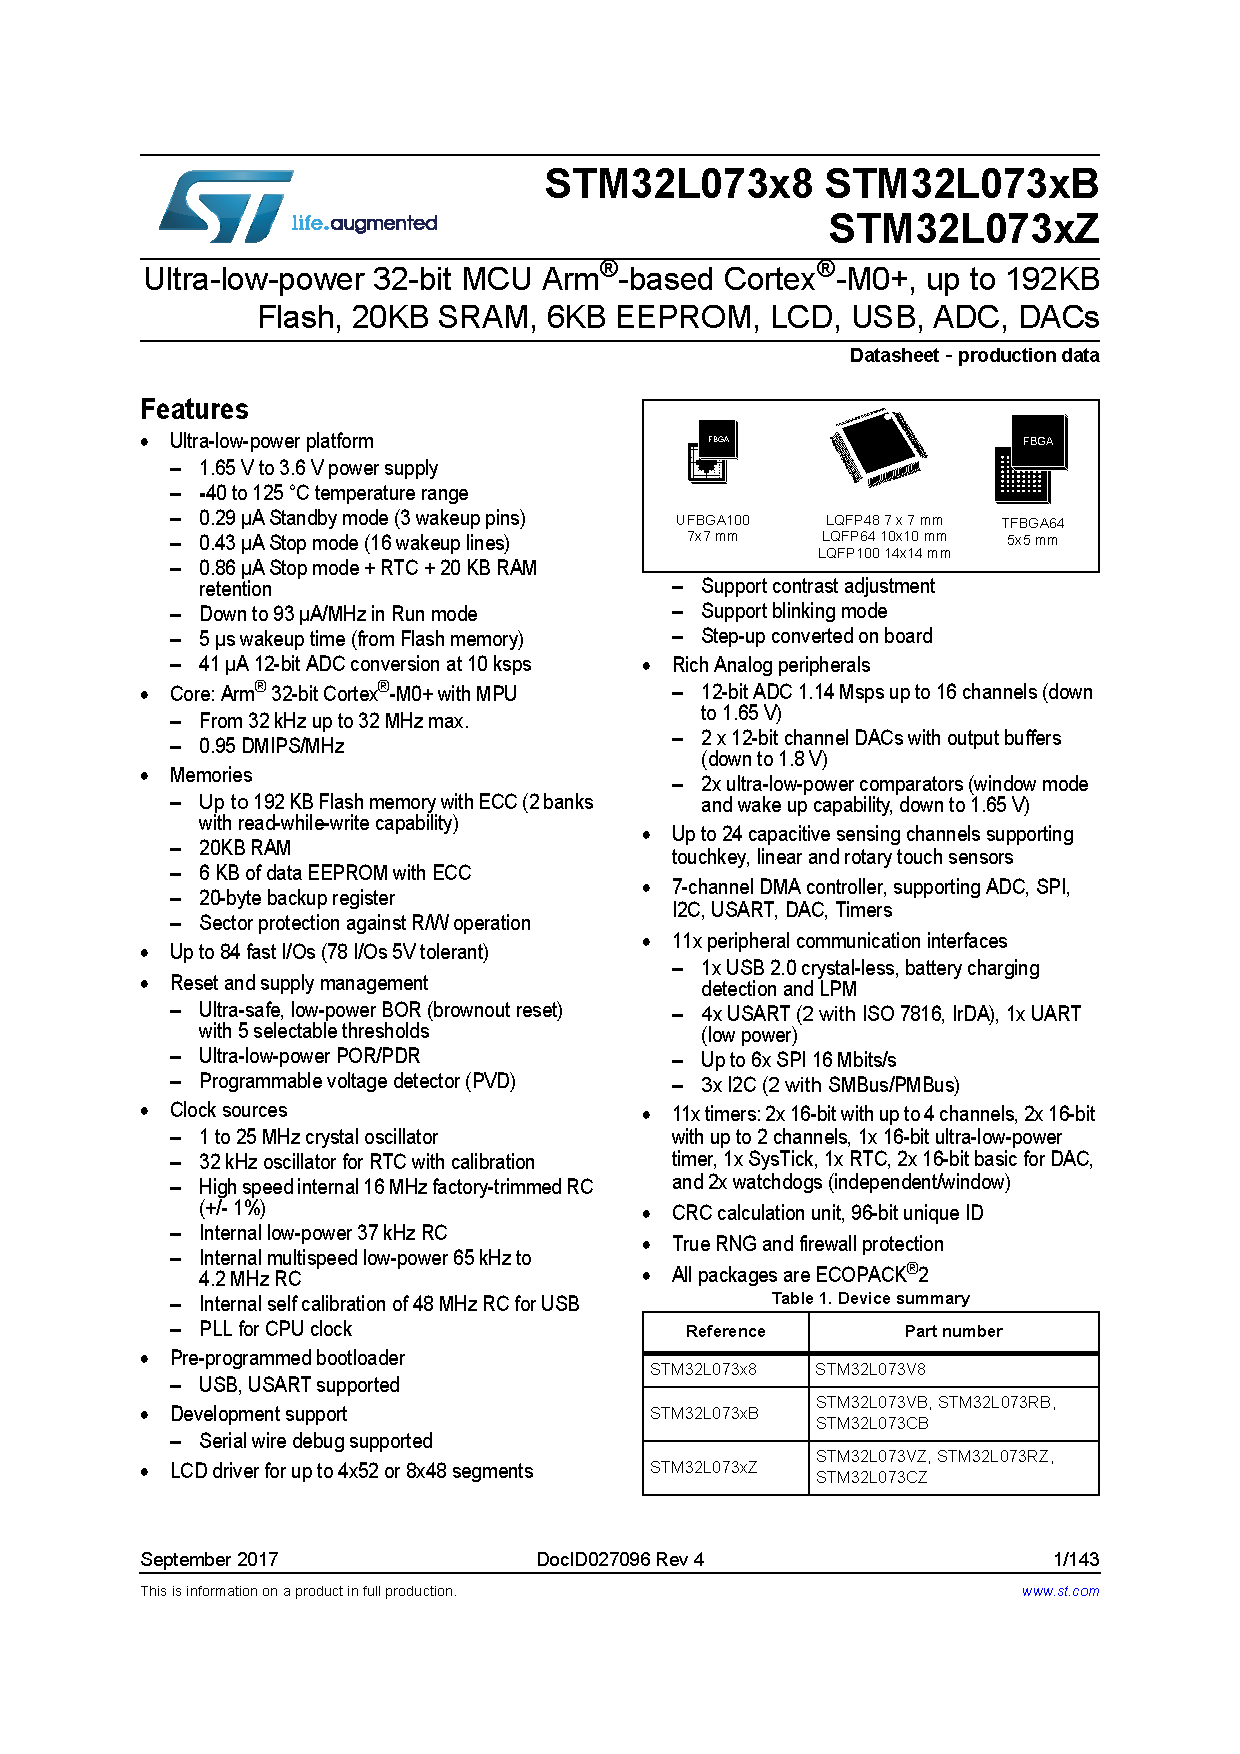
\includegraphics[page=1, angle=0, width=\linewidth]{../Datasheets/stm32l073rz.pdf}
\caption{Kurze Zusammenfassung der Features des STM32L073RZ auf der ersten Seite des Datenblattes}
\end{figure}

\subsection{Debug}

Platzhalter\\Platzhalter\\Platzhalter\\Platzhalter\\Platzhalter\\Platzhalter\\
Platzhalter\\Platzhalter

\begin{figure}[H]\centering
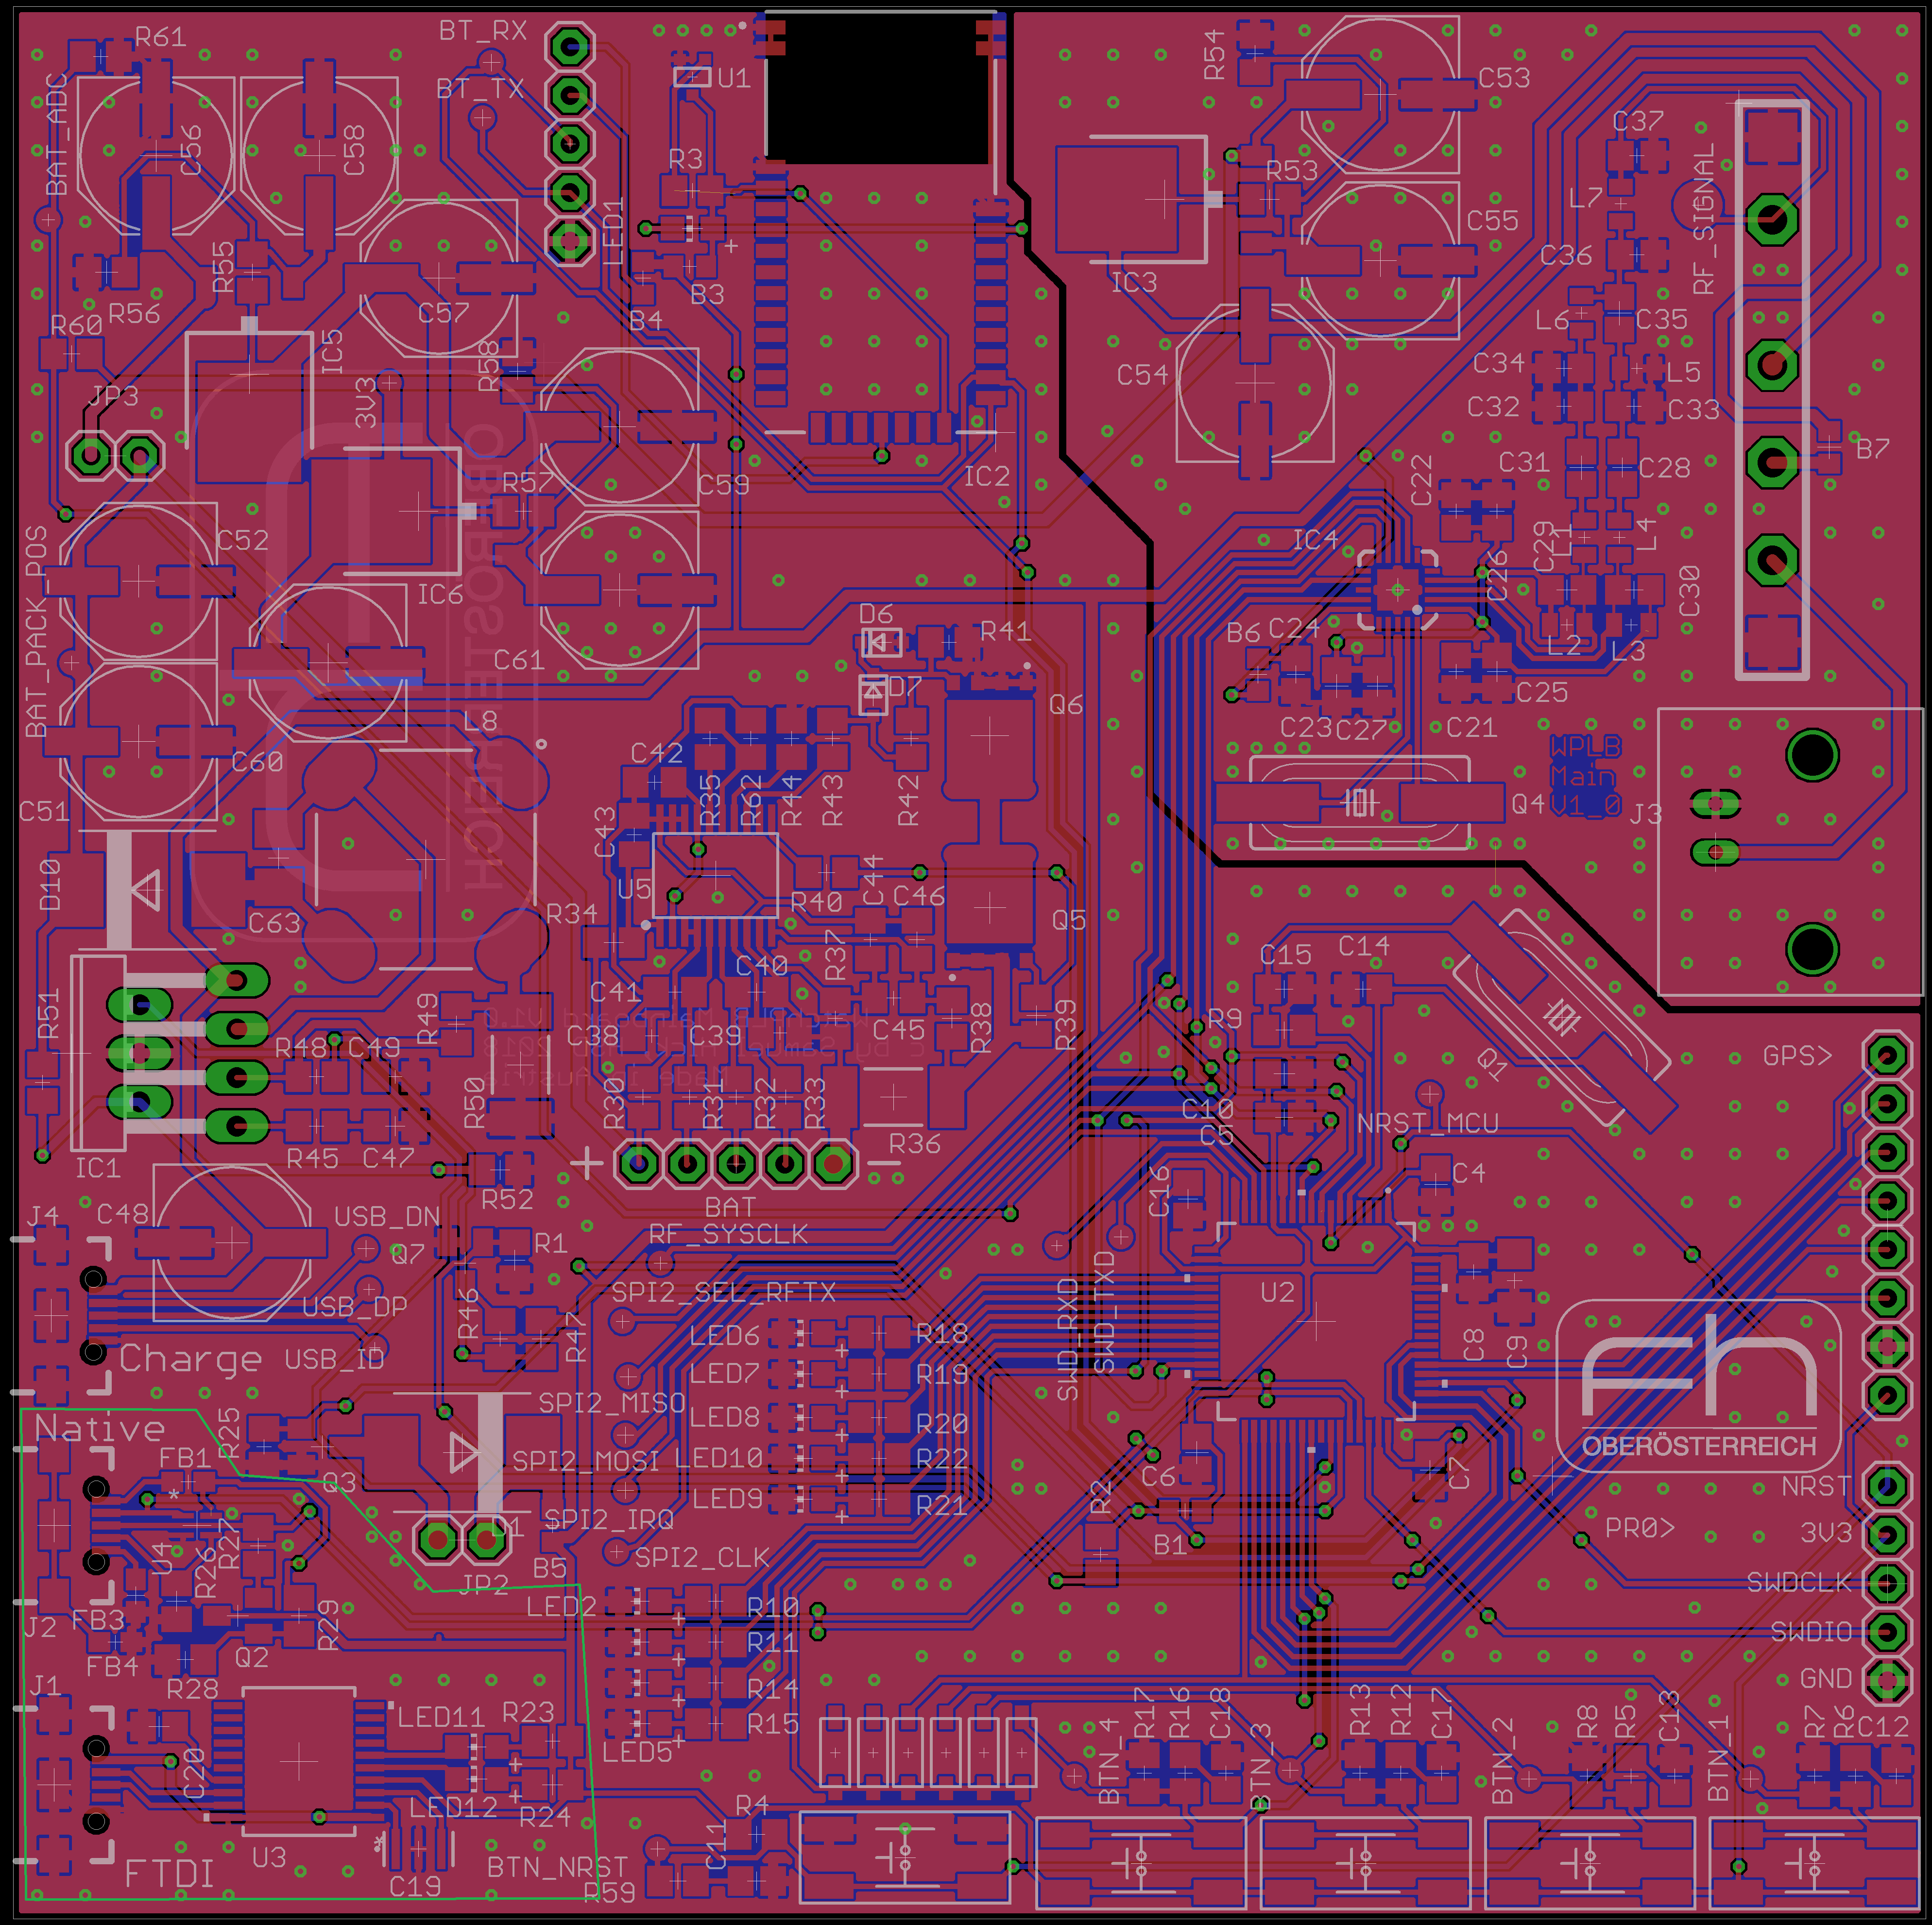
\includegraphics[page=1, angle=0, width=\linewidth]{../Documentation/pics/mainboard_debug.png}
\caption{Hauptplatine, Baugruppe Debug grün umrahmt}
\end{figure}

\begin{figure}[H]\centering
\includegraphics[page=6, angle=90, width=\linewidth]{../eagle/Mainboard/watchplb_mainboard_v1_0.pdf}
\caption{USB-To-UART und USB des STM}
\end{figure}

\subsection{Funk}

Platzhalter\\Platzhalter\\Platzhalter\\Platzhalter\\Platzhalter\\Platzhalter\\
Platzhalter\\Platzhalter

\begin{figure}[H]\centering
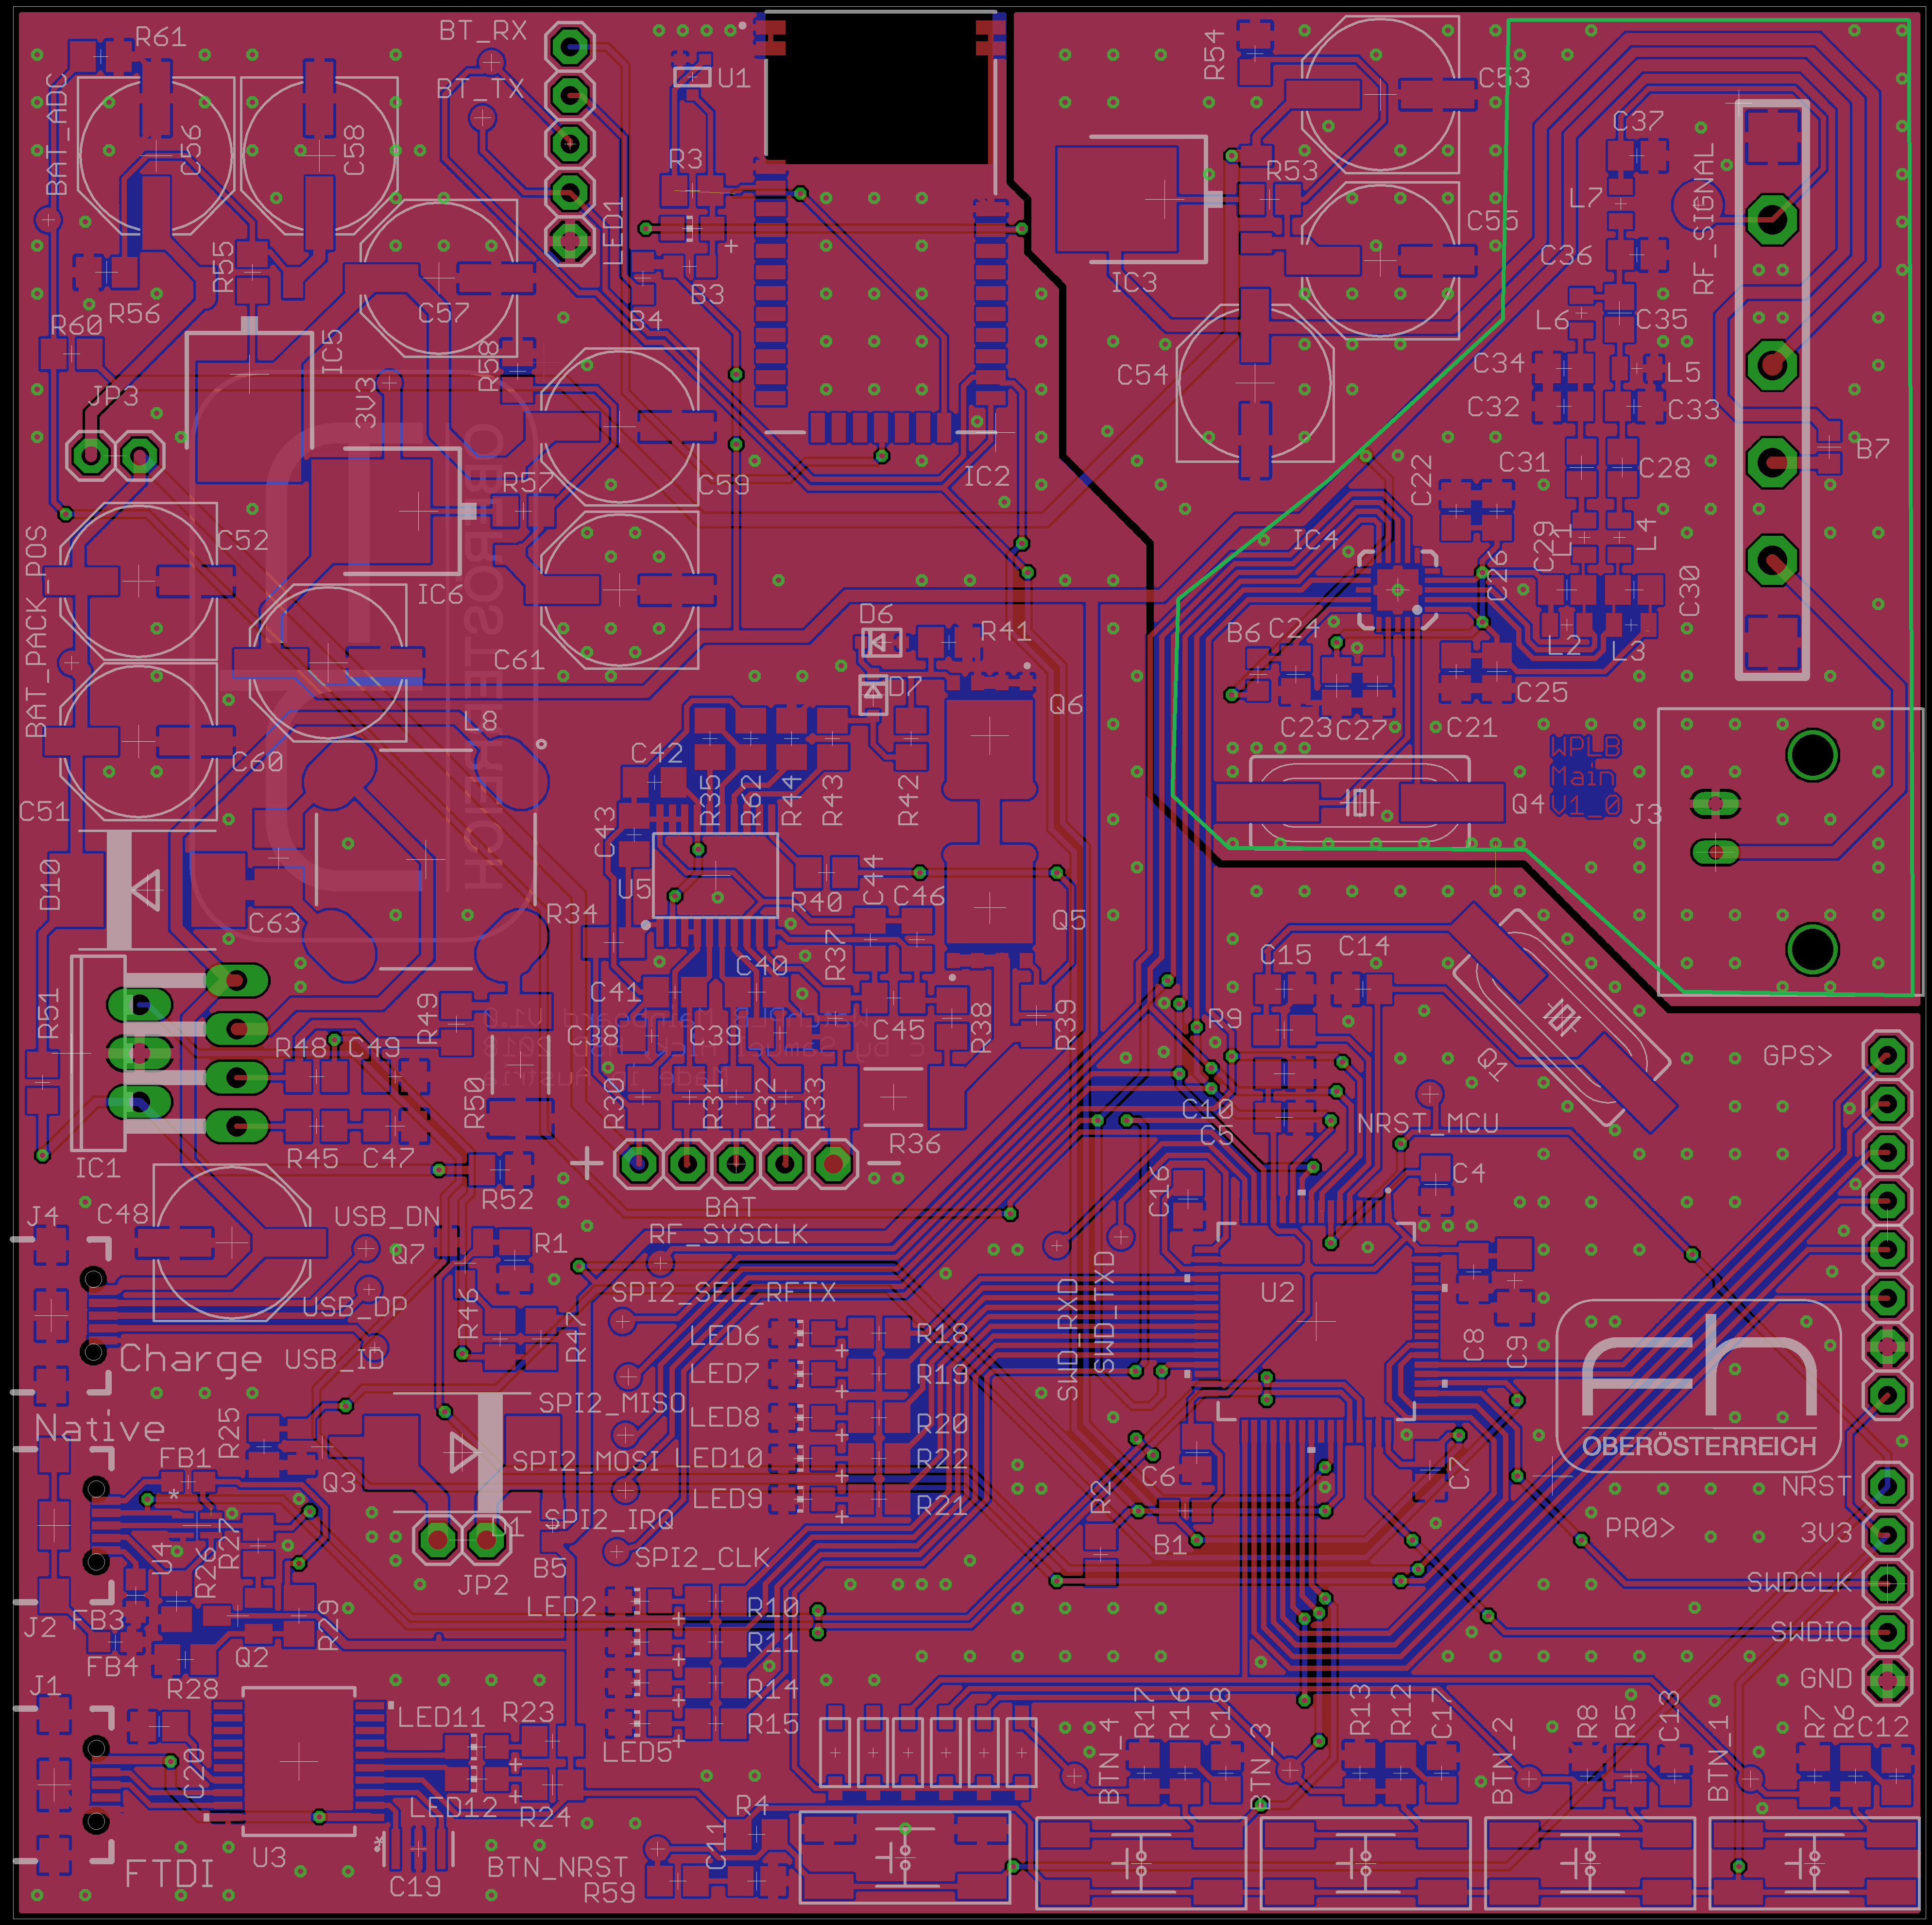
\includegraphics[page=1, angle=0, width=\linewidth]{../Documentation/pics/mainboard_funk.png}
\caption{Hauptplatine, Baugruppe Funk grün umrahmt}
\end{figure}

\begin{figure}[H]\centering
\includegraphics[page=2, angle=90, width=\linewidth]{../eagle/Mainboard/watchplb_mainboard_v1_0.pdf}
\caption{Funk}
\end{figure}

\subsection{Buttons}

Platzhalter\\Platzhalter\\Platzhalter\\Platzhalter\\Platzhalter\\Platzhalter\\
Platzhalter\\Platzhalter

\begin{figure}[H]\centering
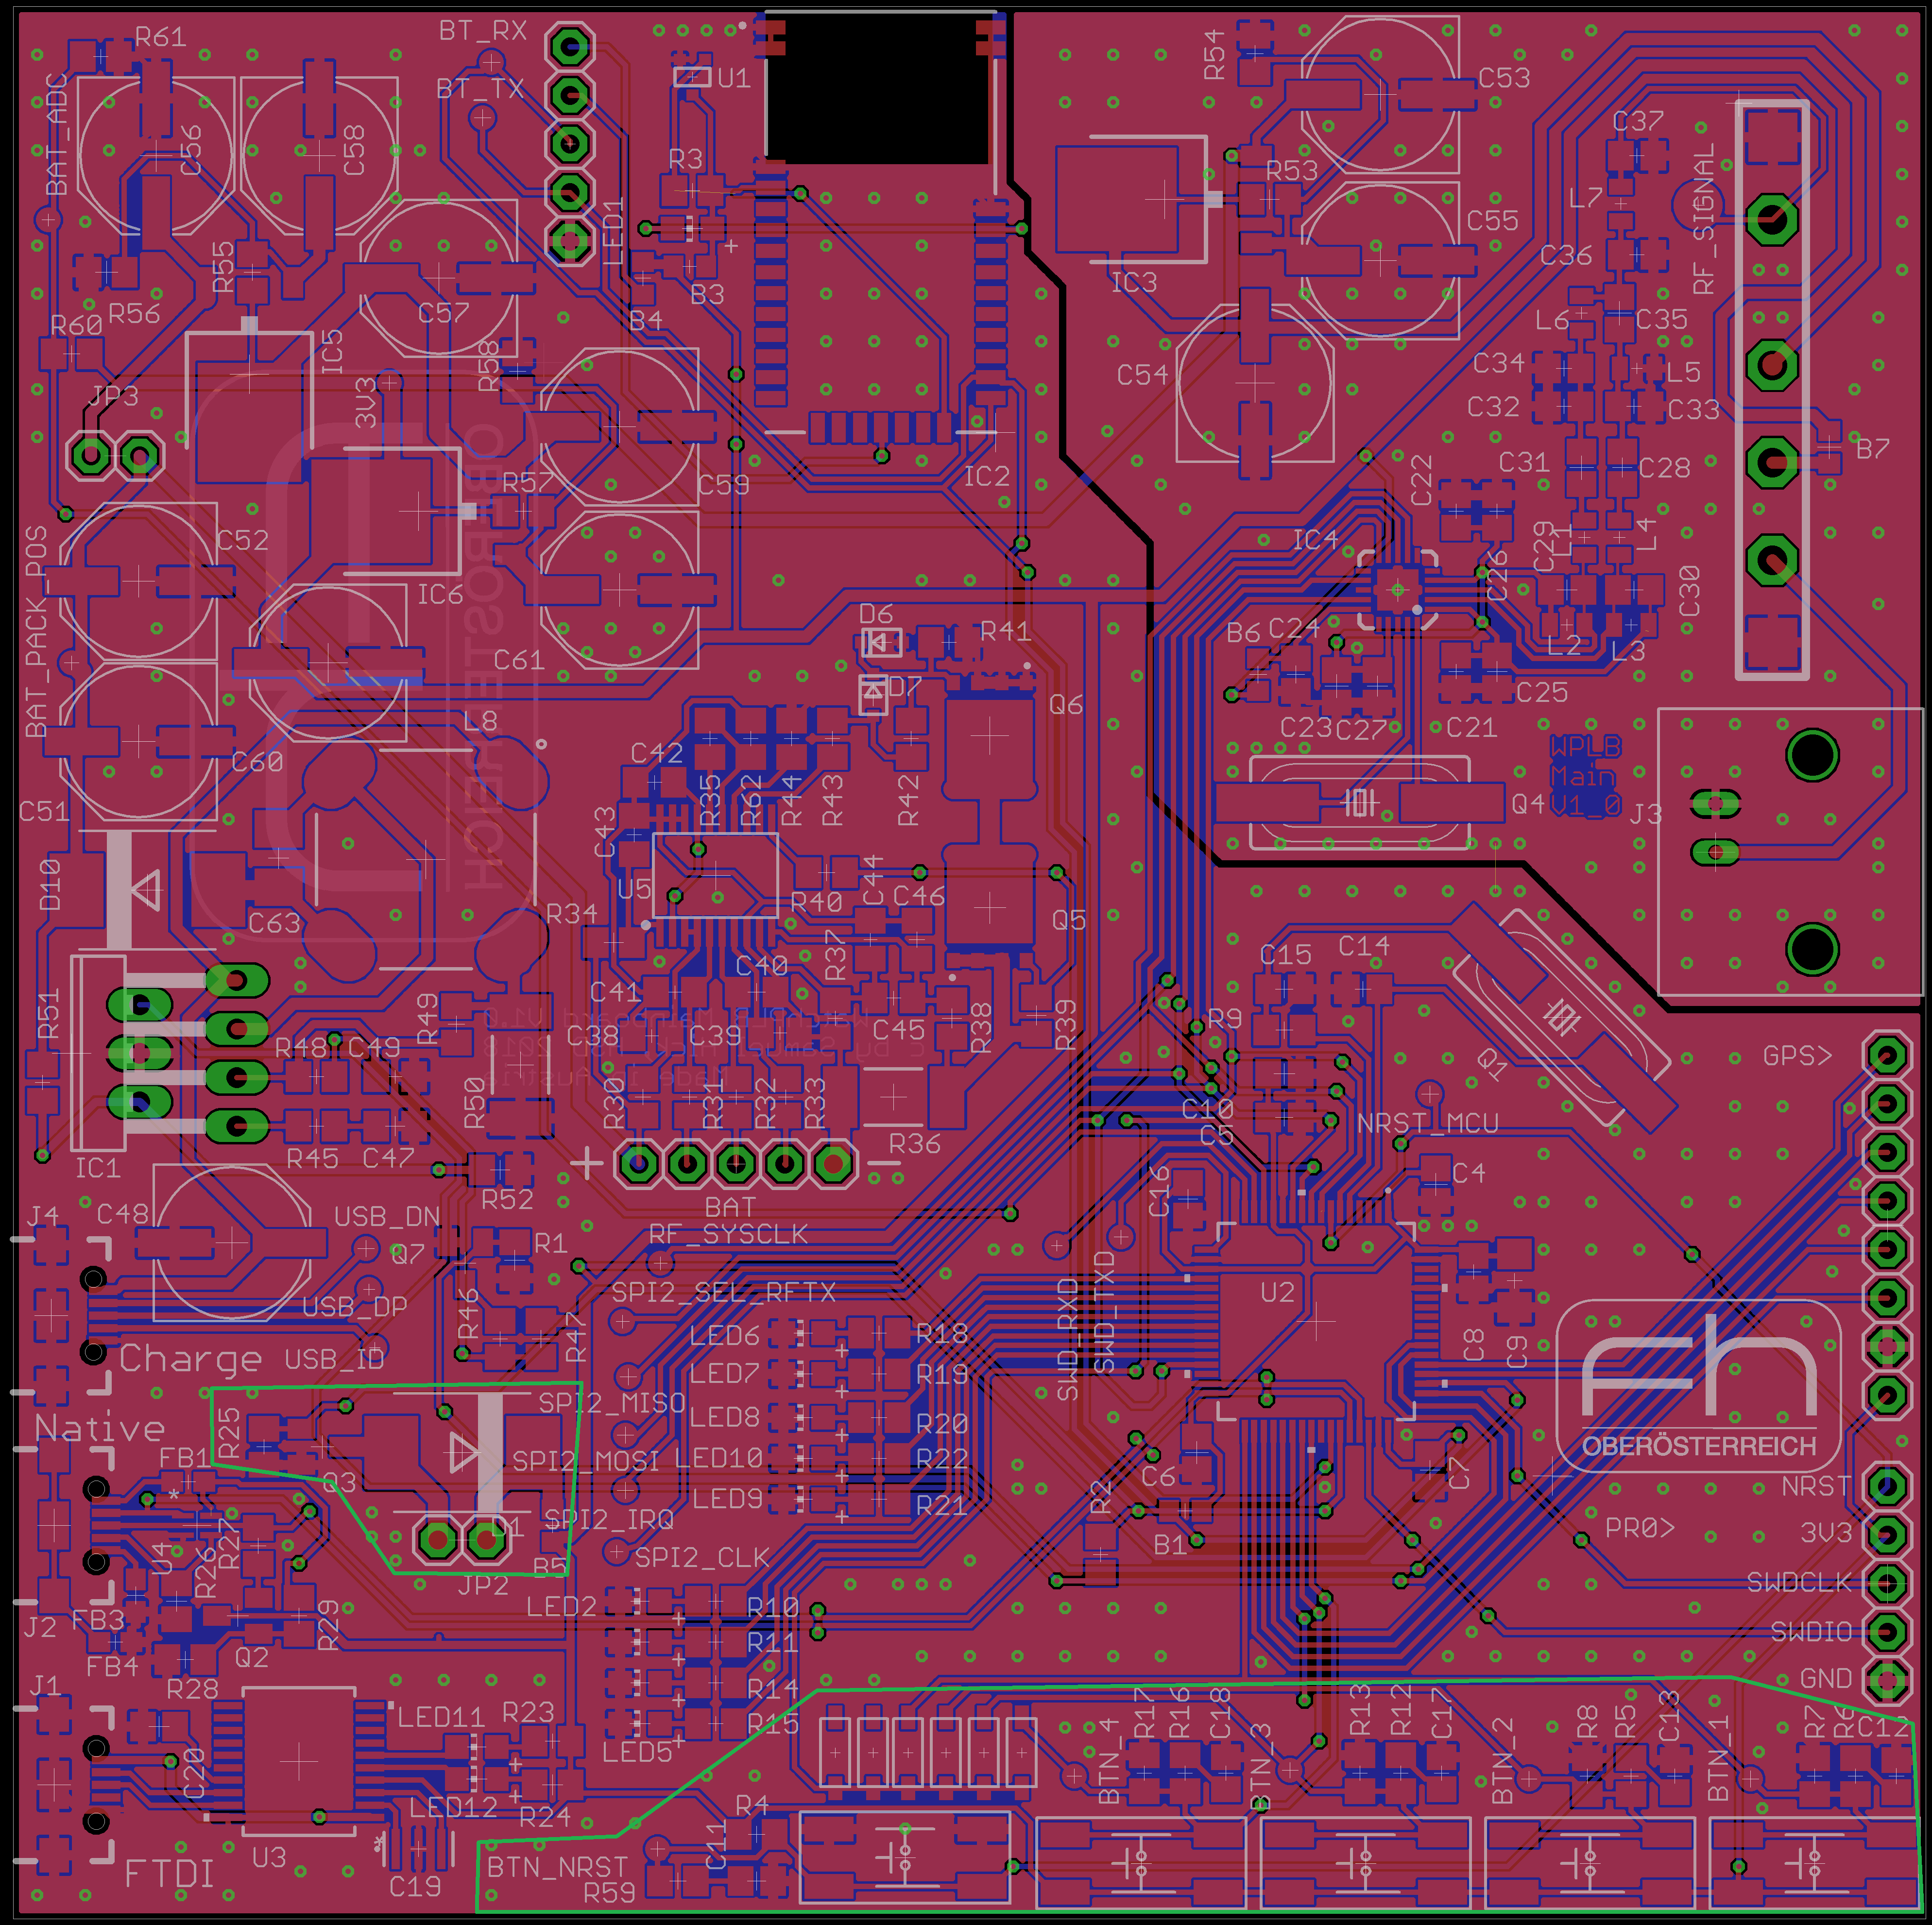
\includegraphics[page=1, angle=0, width=\linewidth]{../Documentation/pics/mainboard_buttons.png}
\caption{Hauptplatine, Baugruppe Buttons grün umrahmt}
\end{figure}

\begin{figure}[H]\centering
\includegraphics[page=3, angle=90, width=\linewidth]{../eagle/Mainboard/watchplb_mainboard_v1_0.pdf}
\caption{Taster, WakeUp, Vibrationsmotor}
\end{figure}

\subsection{Bluetooth}

Platzhalter\\Platzhalter\\Platzhalter\\Platzhalter\\Platzhalter\\Platzhalter\\
Platzhalter\\Platzhalter

\begin{figure}[H]\centering
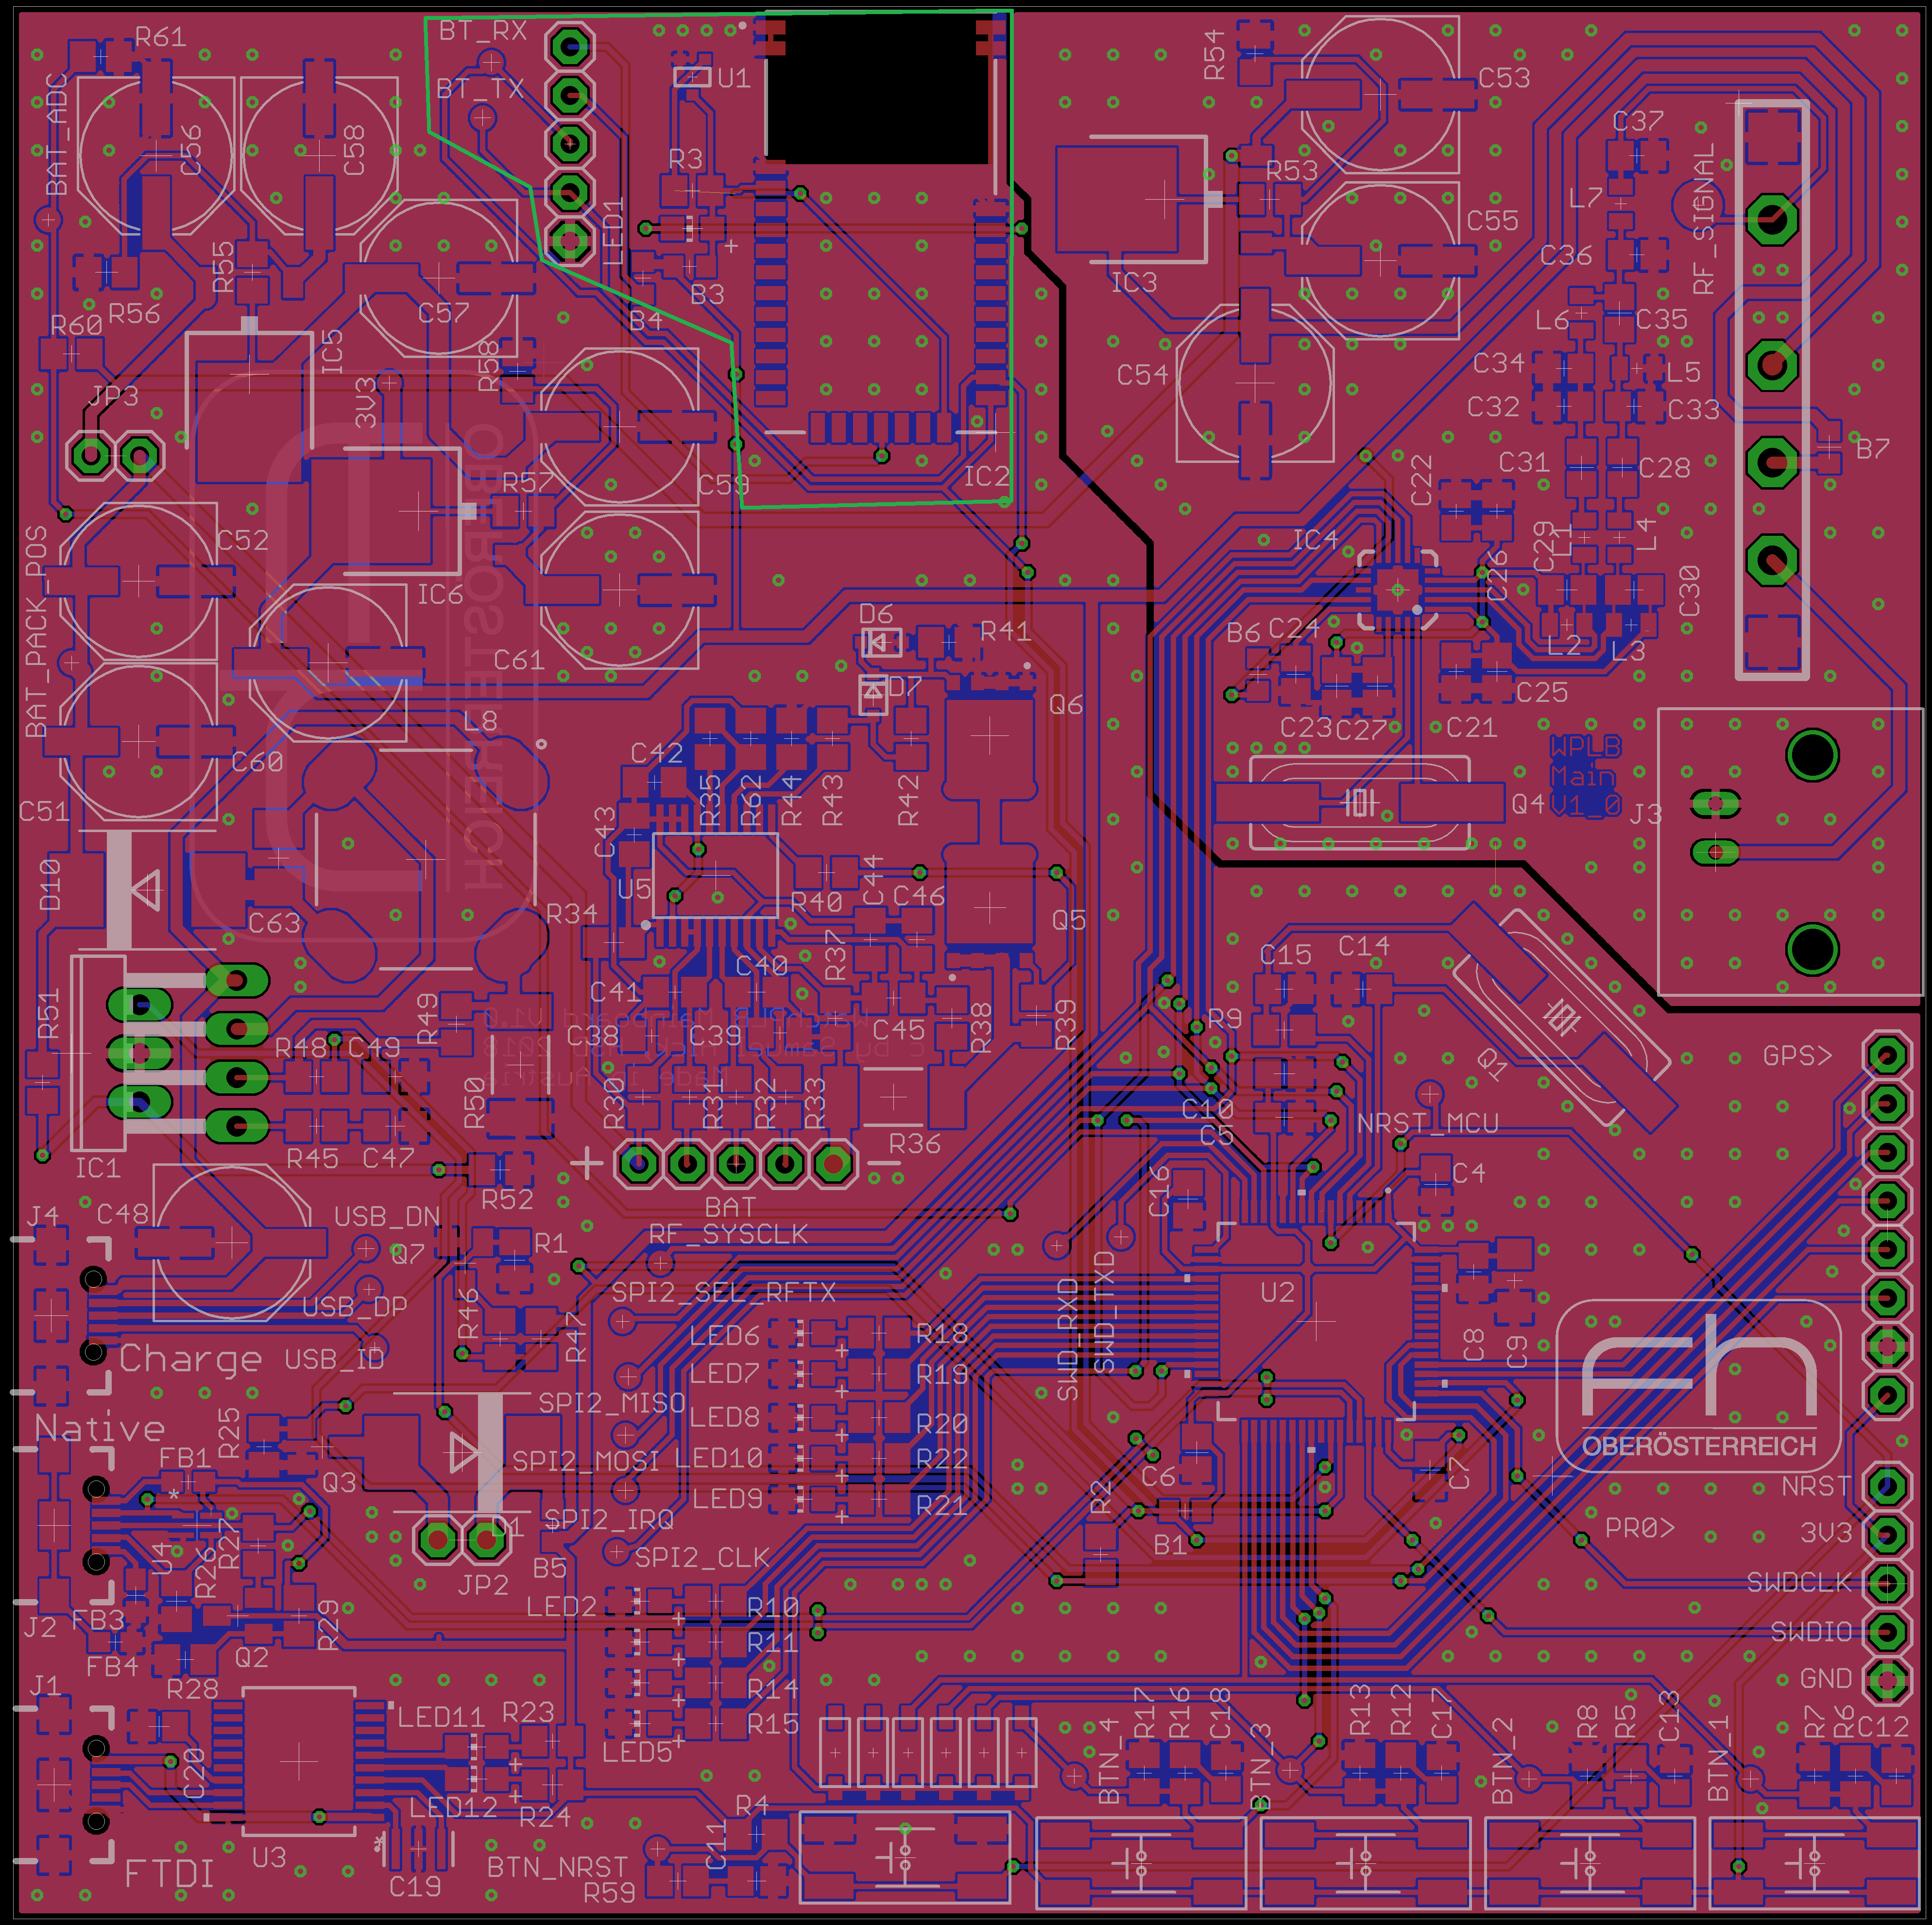
\includegraphics[page=1, angle=0, width=\linewidth]{../Documentation/pics/mainboard_bluetooth.png}
\caption{Hauptplatine, Baugruppe Bluetooth grün umrahmt}
\end{figure}

\begin{figure}[H]\centering
\includegraphics[page=4, angle=90, width=\linewidth]{../eagle/Mainboard/watchplb_mainboard_v1_0.pdf}
\caption{Bluetooth-Modul}
\end{figure}

\subsection{Charge}

Platzhalter\\Platzhalter\\Platzhalter\\Platzhalter\\Platzhalter\\Platzhalter\\
Platzhalter\\Platzhalter

\begin{figure}[H]\centering
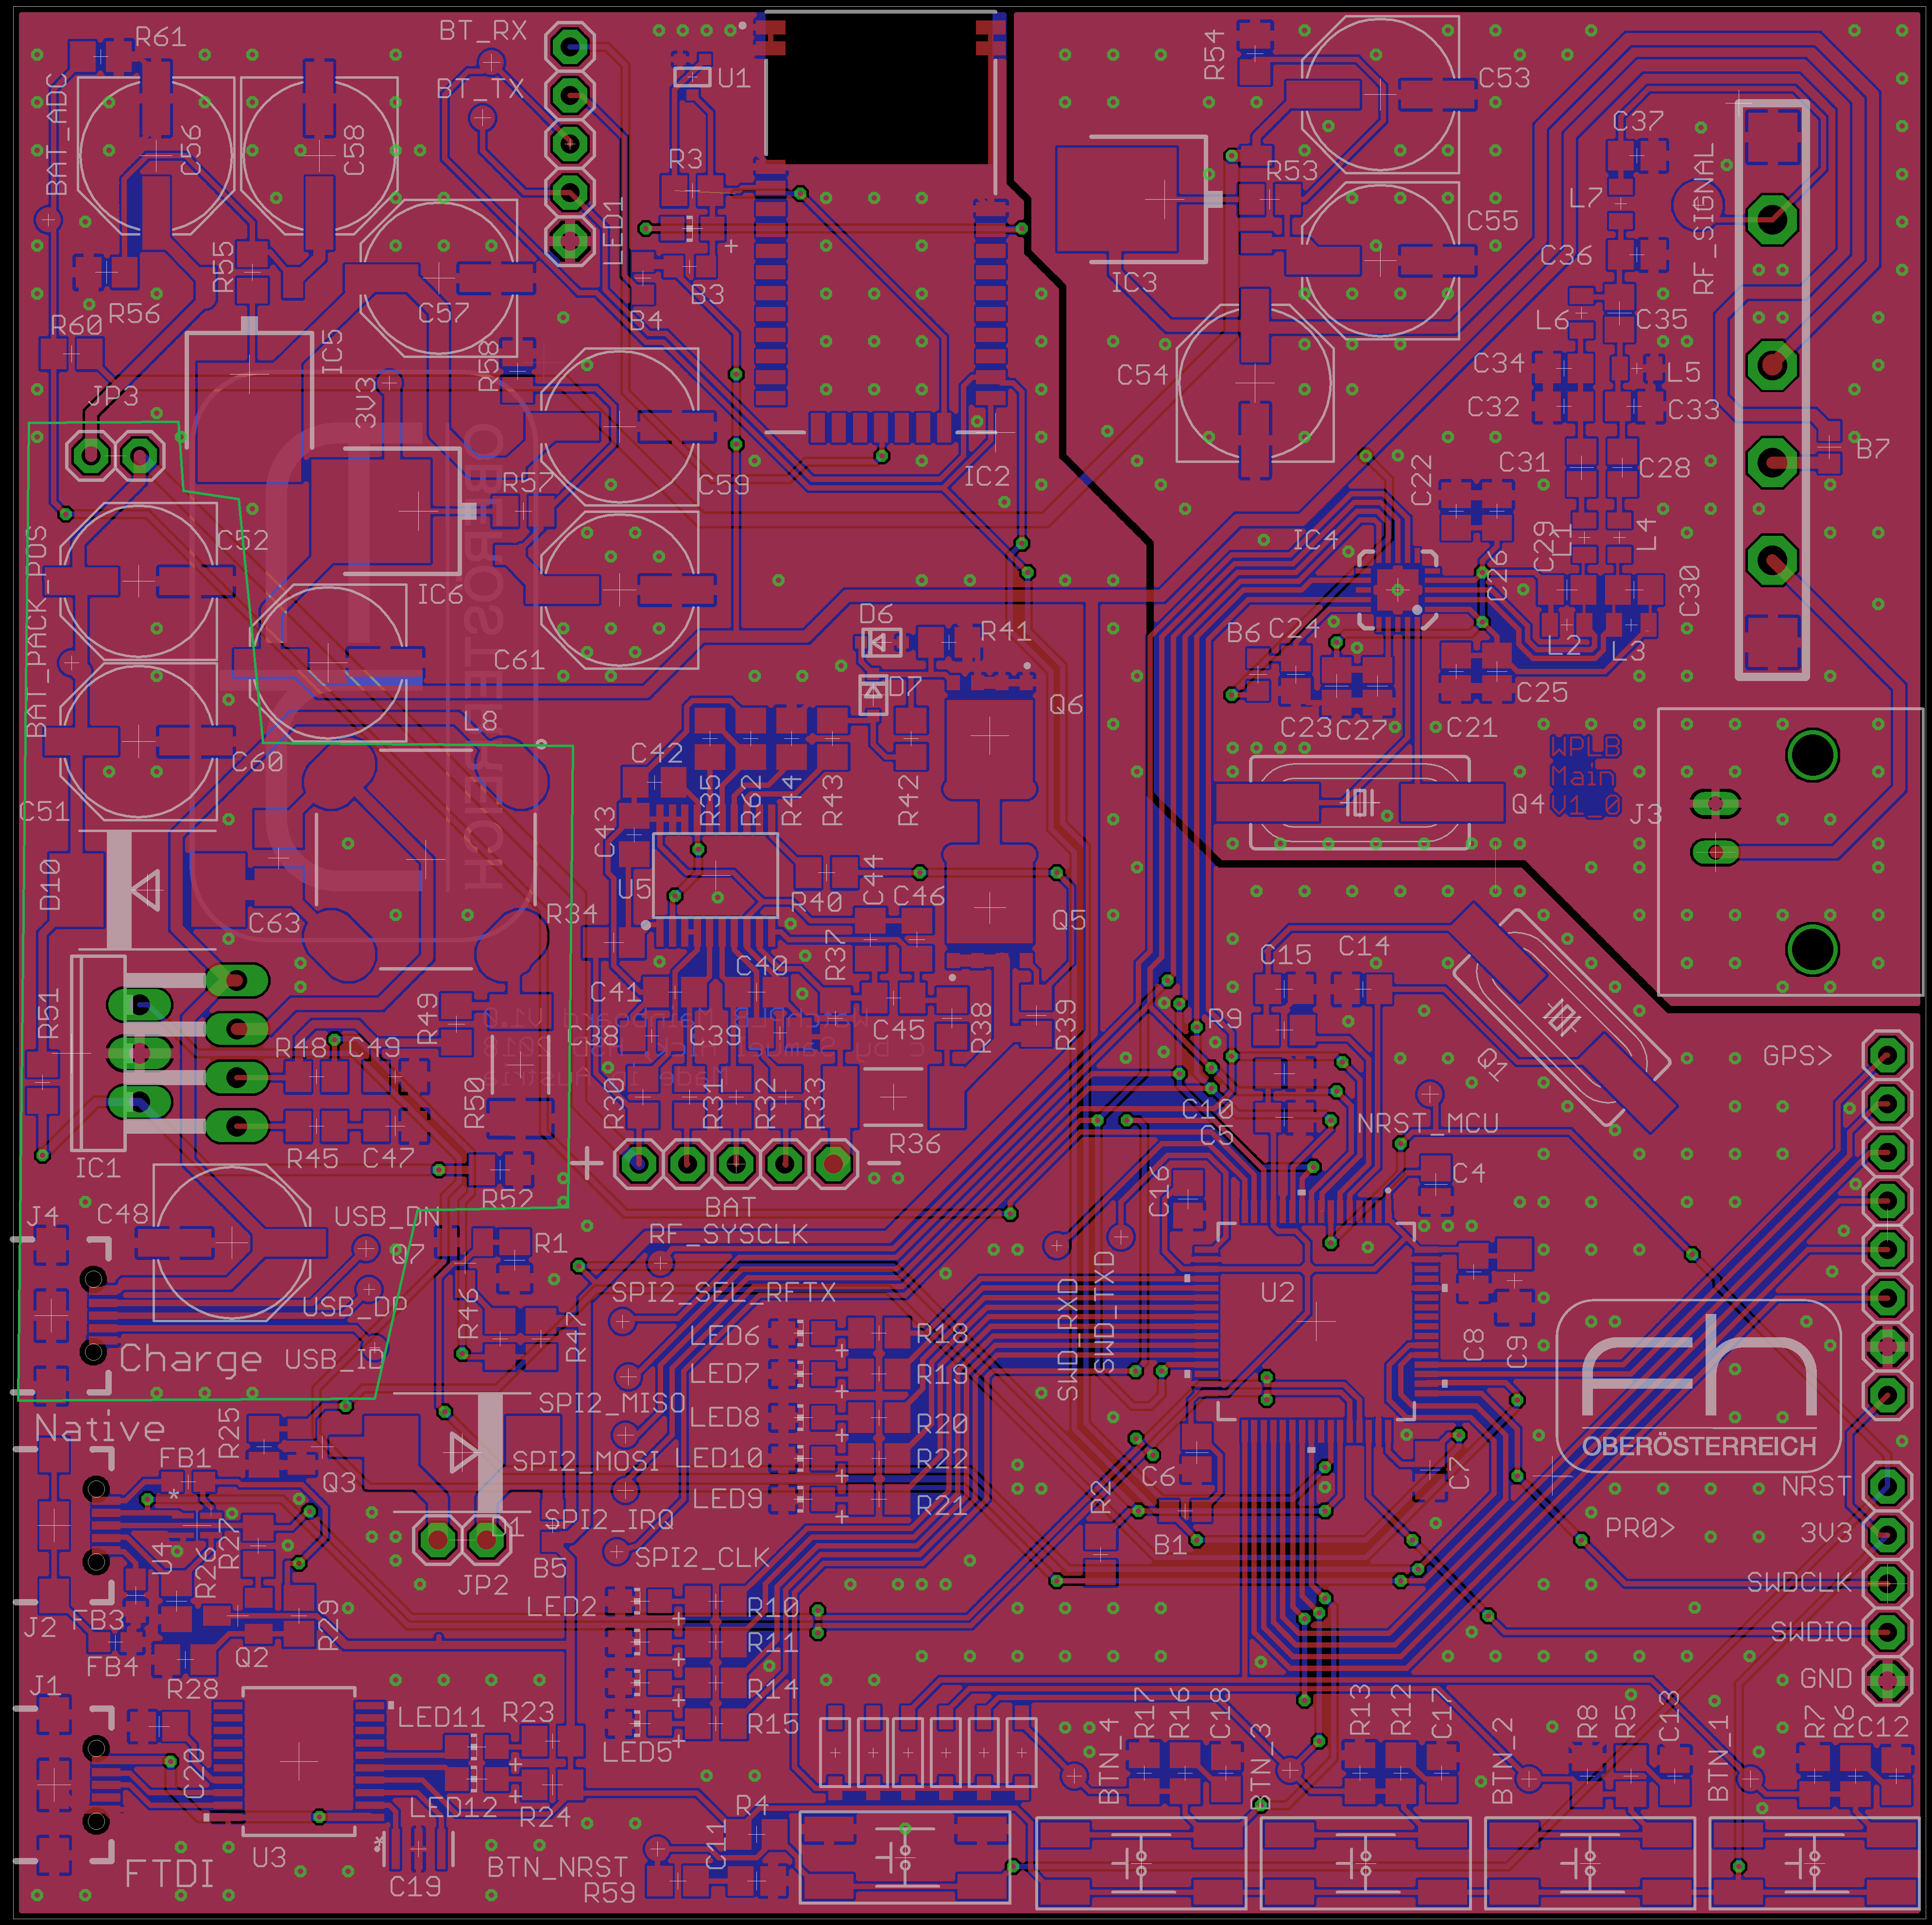
\includegraphics[page=1, angle=0, width=\linewidth]{../Documentation/pics/mainboard_charge.png}
\caption{Hauptplatine, Baugruppe Charge umrahmt}
\end{figure}

\begin{figure}[H]\centering
\includegraphics[page=5, angle=90, width=\linewidth]{../eagle/Mainboard/watchplb_mainboard_v1_0.pdf}
\caption{Akkuladeschaltung}
\end{figure}

\subsection{Battery Protection}

Platzhalter\\Platzhalter\\Platzhalter\\Platzhalter\\Platzhalter\\Platzhalter\\
Platzhalter\\Platzhalter

\begin{figure}[H]\centering
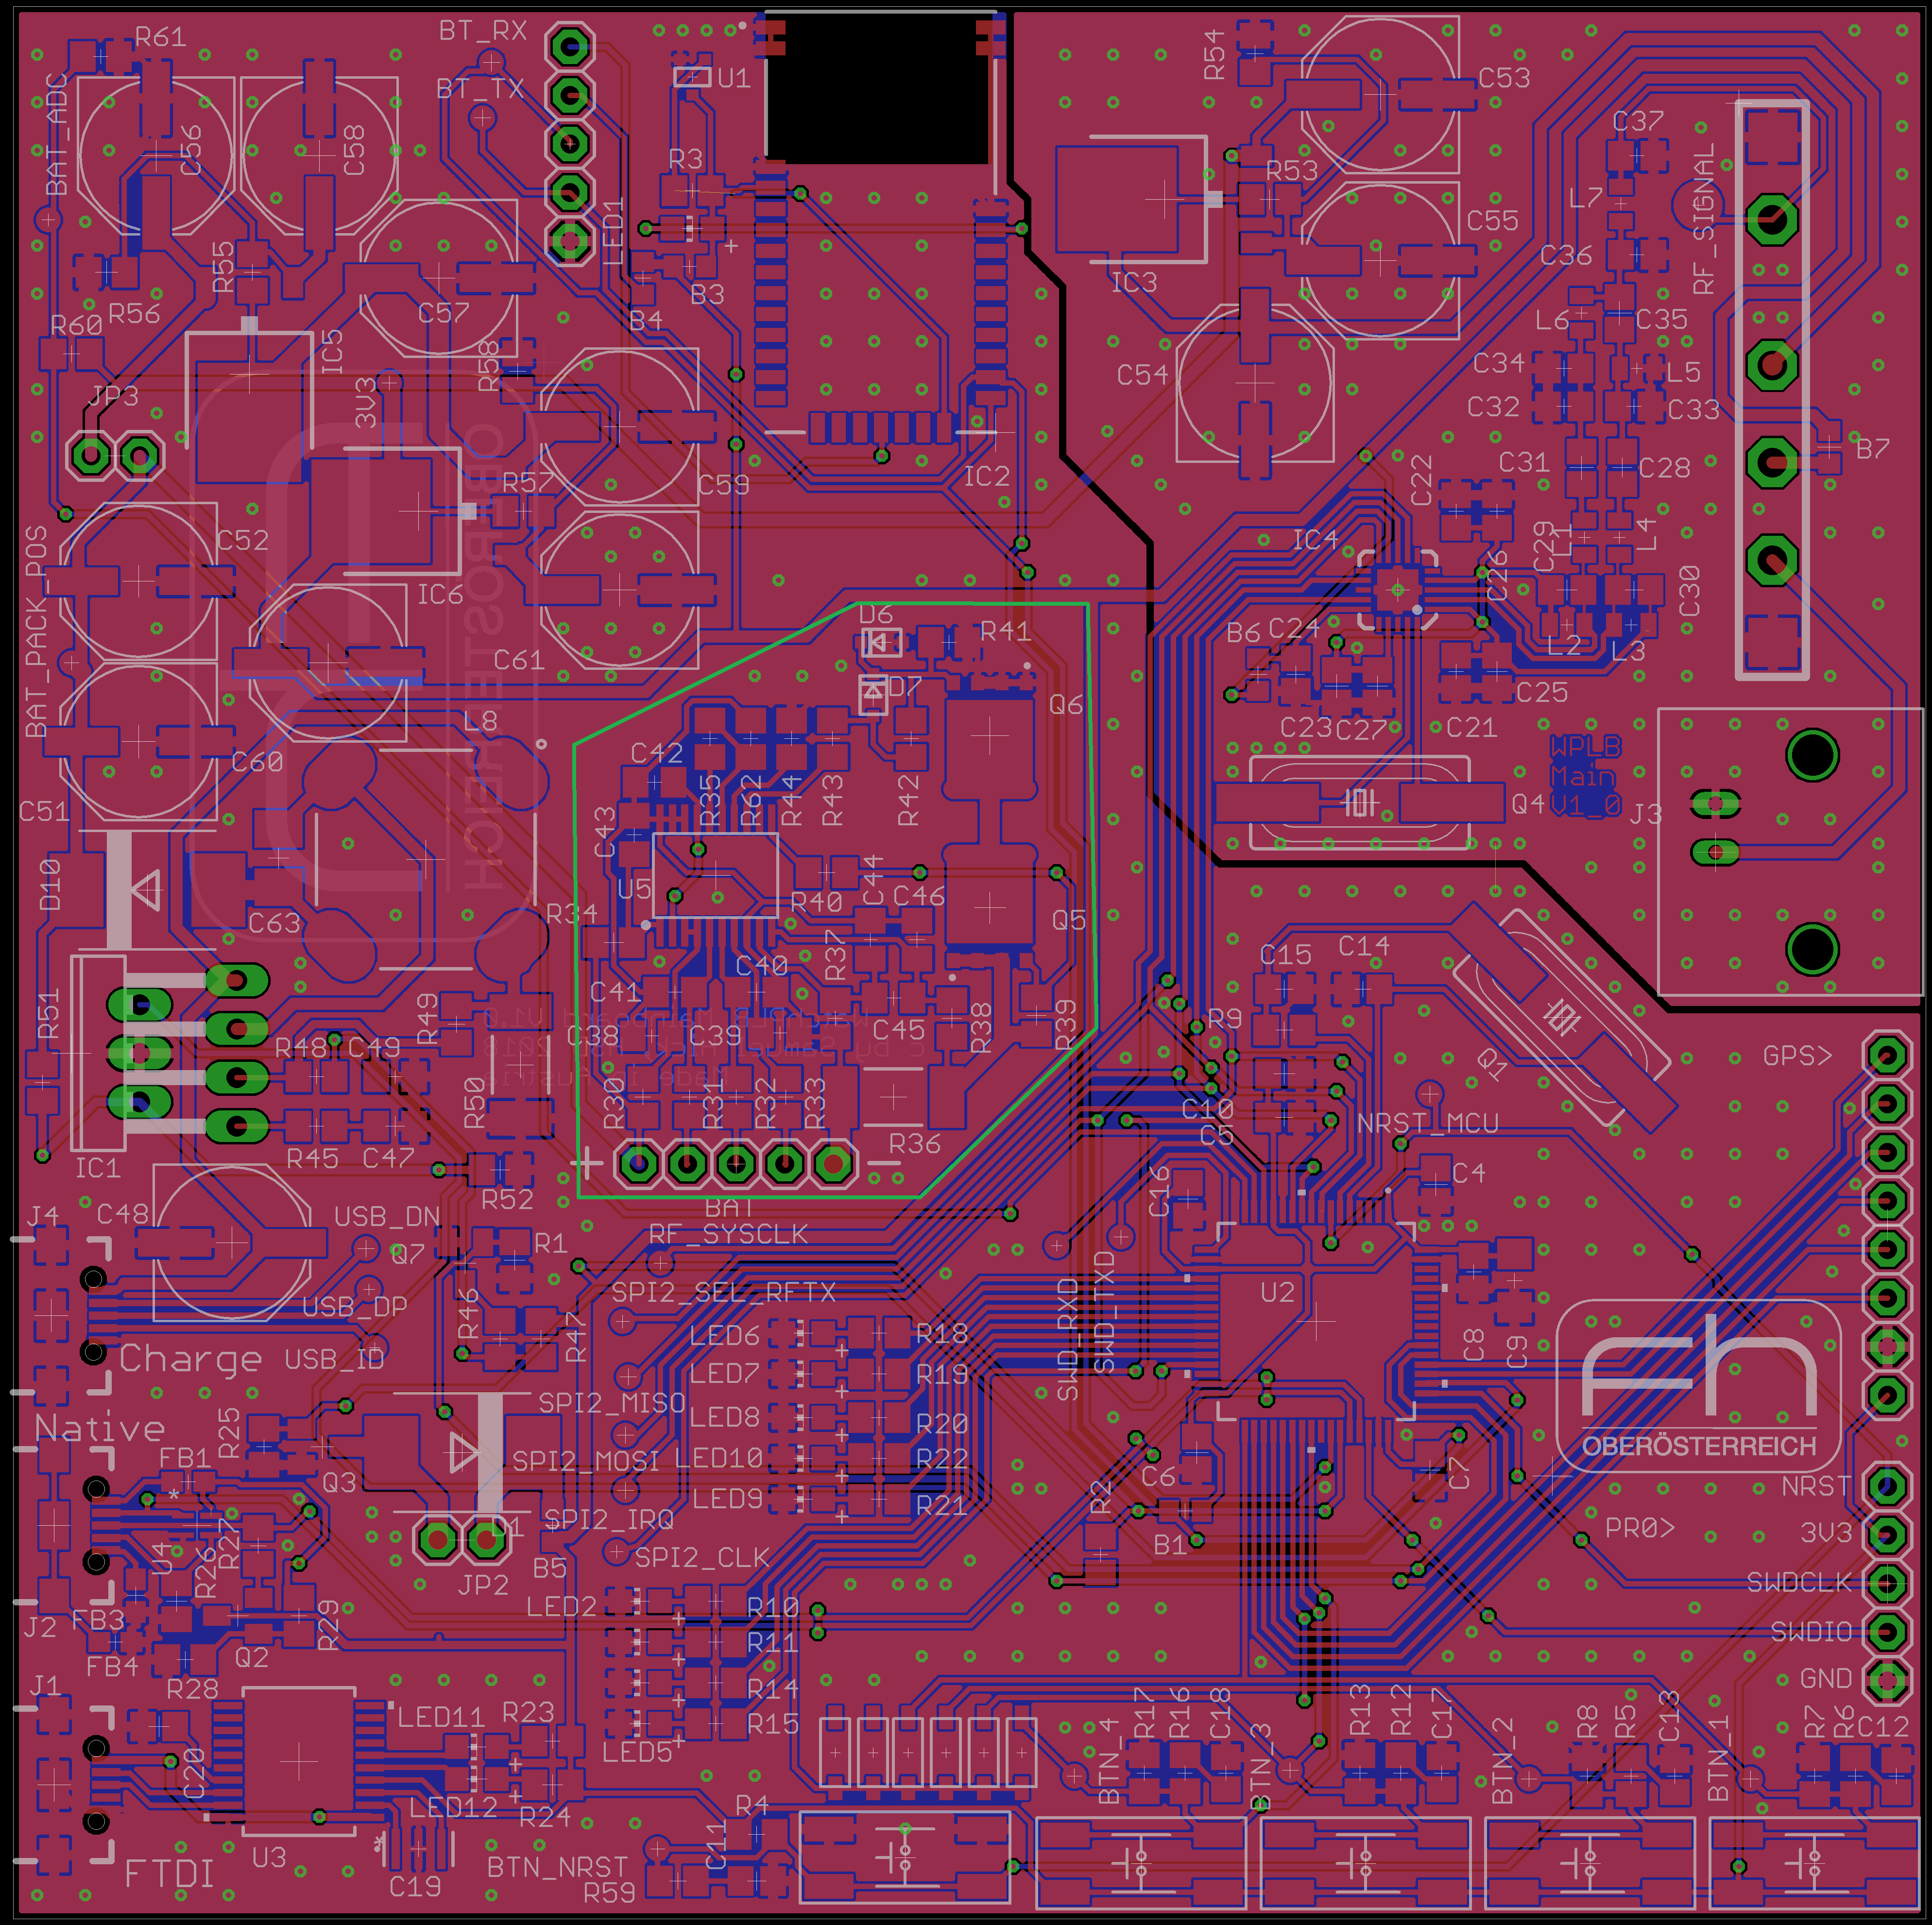
\includegraphics[page=1, angle=0, width=\linewidth]{../Documentation/pics/mainboard_batprot.png}
\caption{Hauptplatine, Baugruppe Battery Protection umrahmt}
\end{figure}

\begin{figure}[H]\centering
\includegraphics[page=7, angle=90, width=\linewidth]{../eagle/Mainboard/watchplb_mainboard_v1_0.pdf}
\caption{Lithium-Ionen-Akku Schutzschaltung}
\end{figure}

\subsection{Voltage Regulator}

Platzhalter\\Platzhalter\\Platzhalter\\Platzhalter\\Platzhalter\\Platzhalter\\
Platzhalter\\Platzhalter

\begin{figure}[H]\centering
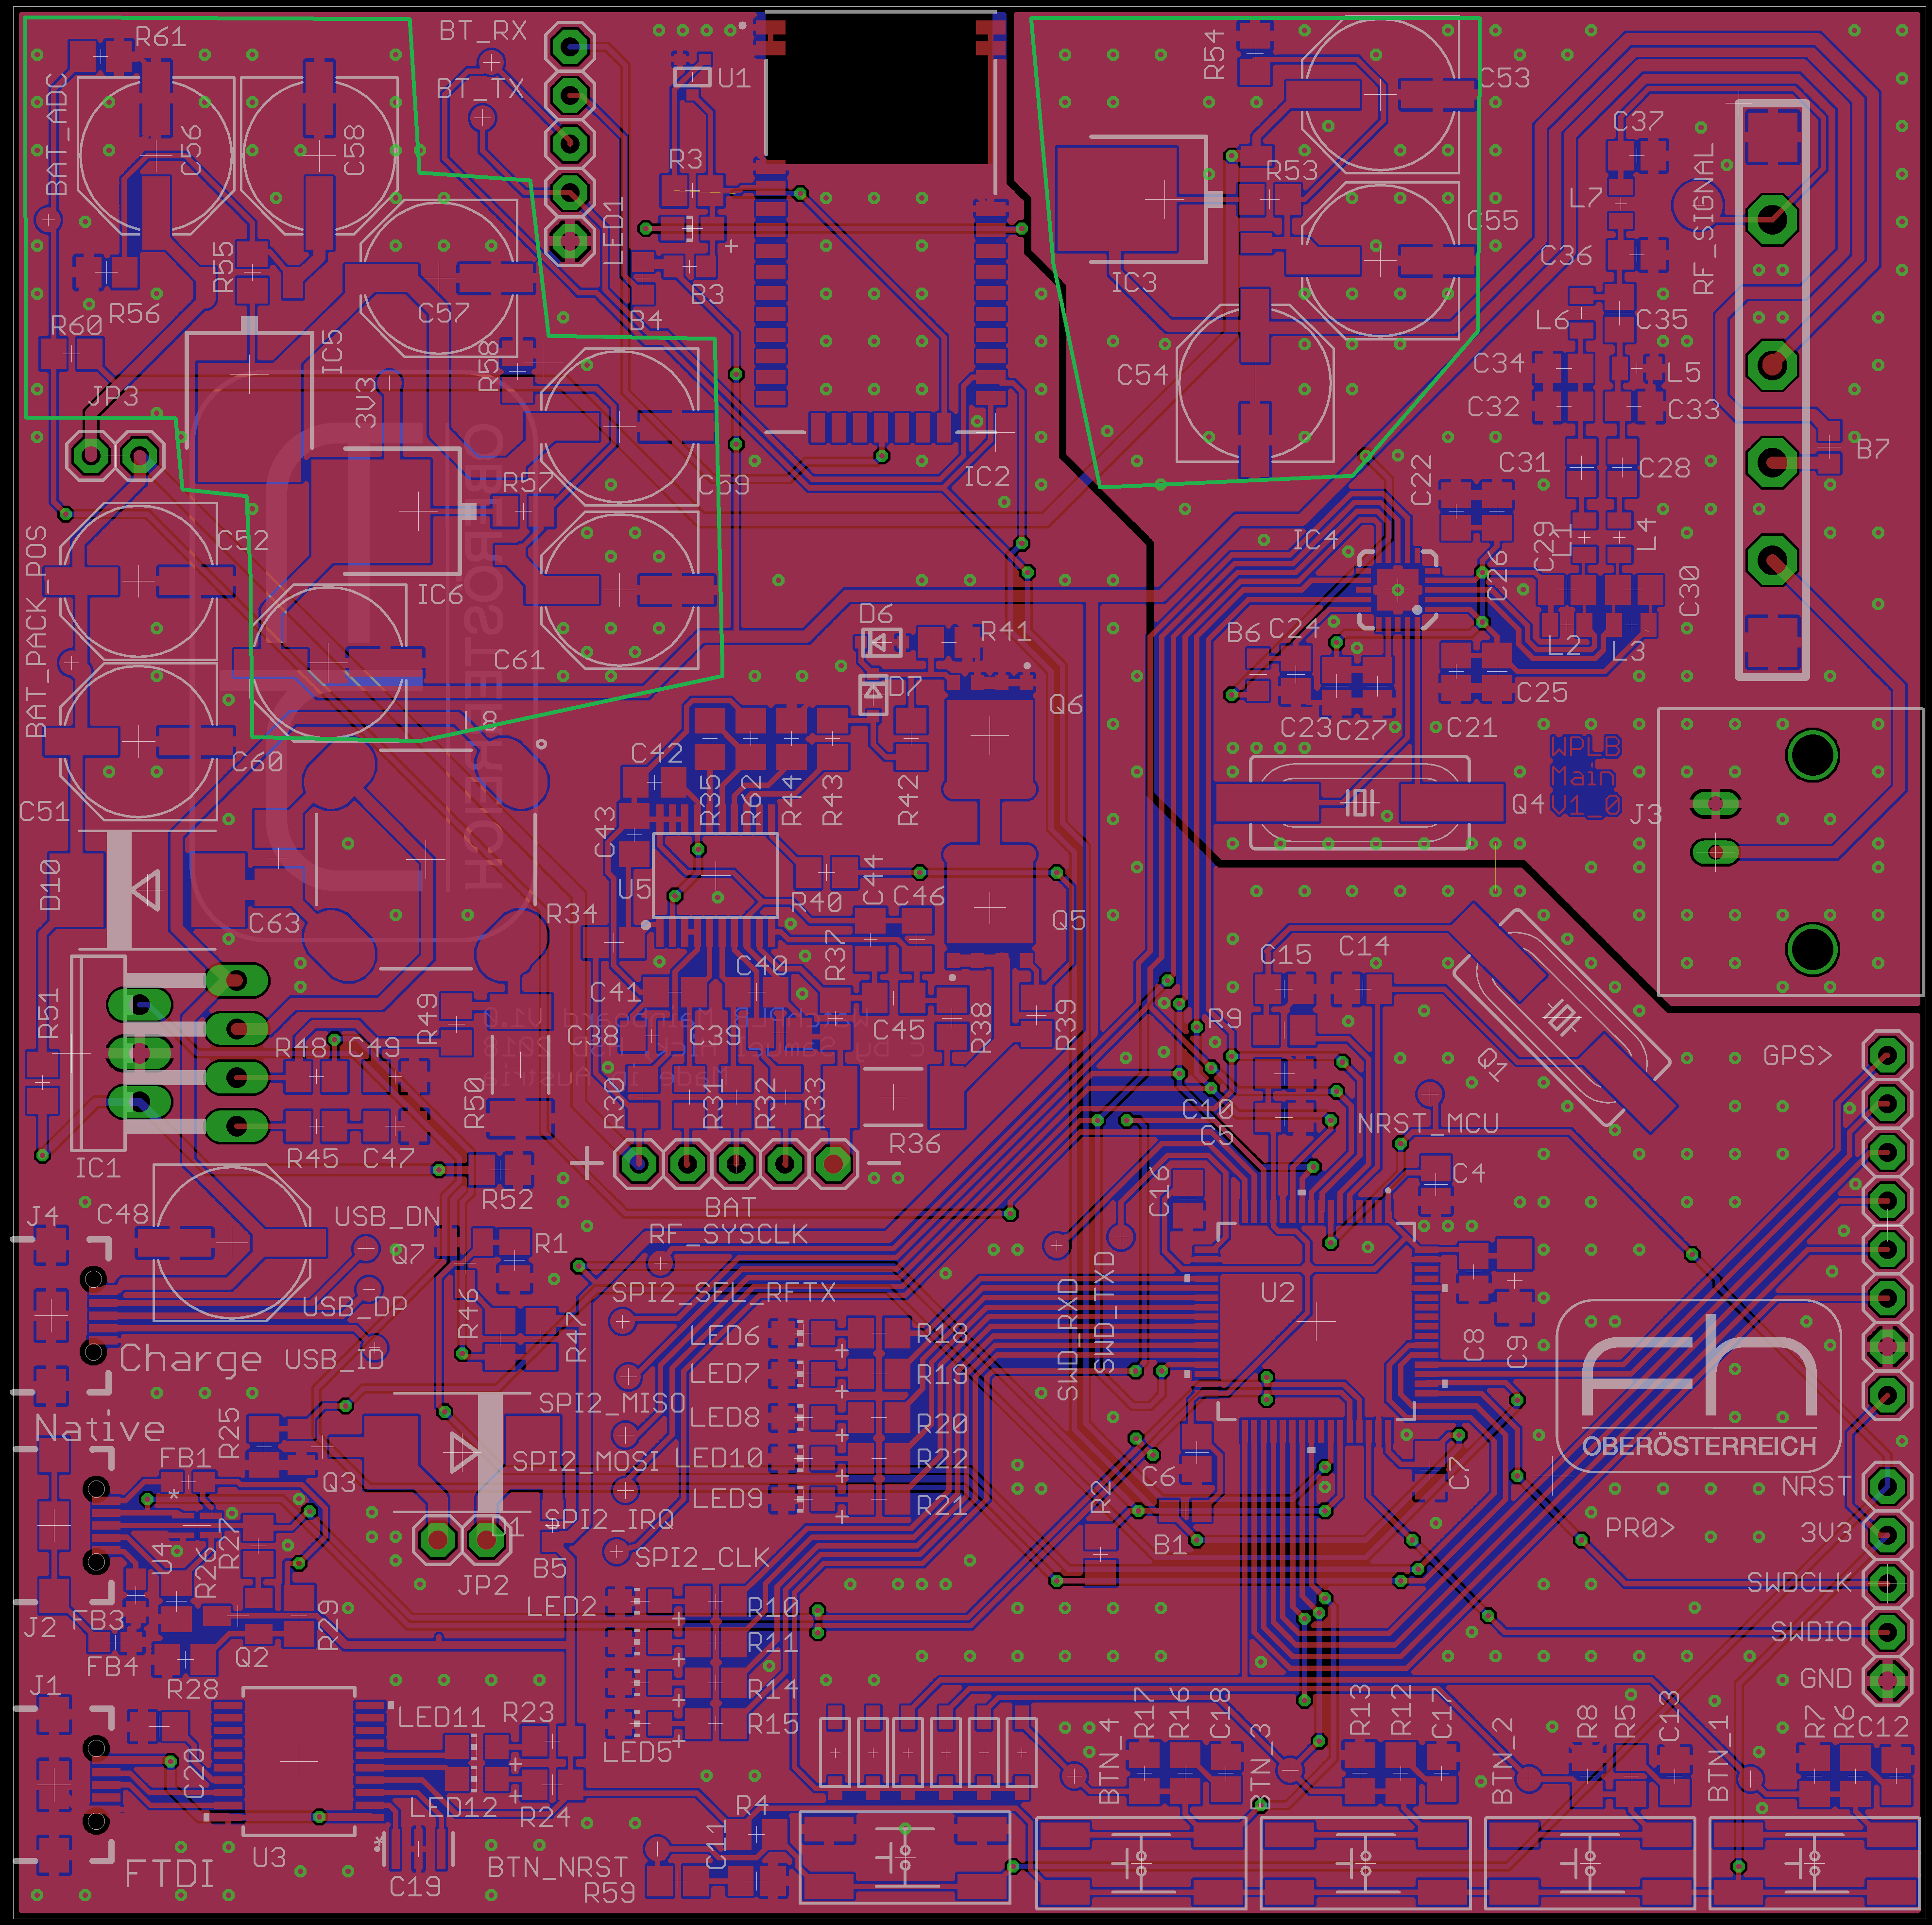
\includegraphics[page=1, angle=0, width=\linewidth]{../Documentation/pics/mainboard_vreg.png}
\caption{Hauptplatine, Baugruppe VREG umrahmt}
\end{figure}

\begin{figure}[H]\centering
\includegraphics[page=8, angle=90, width=\linewidth]{../eagle/Mainboard/watchplb_mainboard_v1_0.pdf}
\caption{Spannungsregler}
\end{figure}

\section{GPS-Board}

Platzhalter\\Platzhalter\\Platzhalter\\Platzhalter\\Platzhalter\\
Platzhalter\\Platzhalter\\Platzhalter\\Platzhalter\\Platzhalter\\
Platzhalter\\Platzhalter\\Platzhalter\\Platzhalter\\Platzhalter\\
Platzhalter\\Platzhalter\\Platzhalter\\Platzhalter\\Platzhalter\\

\begin{figure}[H]\centering
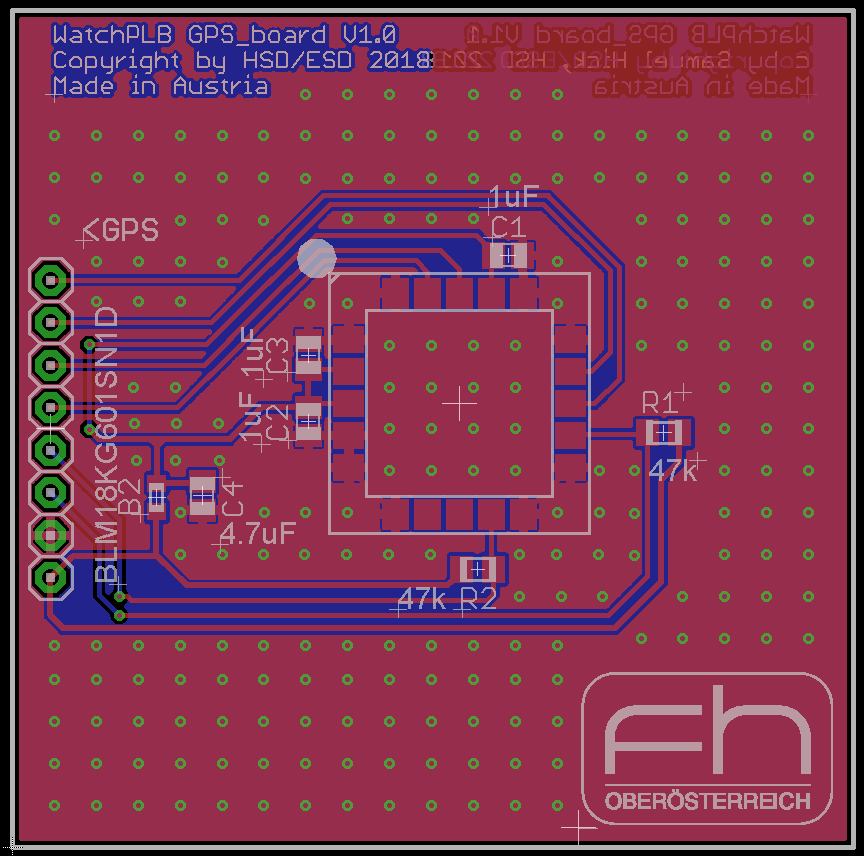
\includegraphics[page=1, angle=0, scale=0.4]{../Documentation/pics/gpsboard.png}
\caption{Platine des GPS-Moduls}
\end{figure}

\begin{figure}[H]\centering
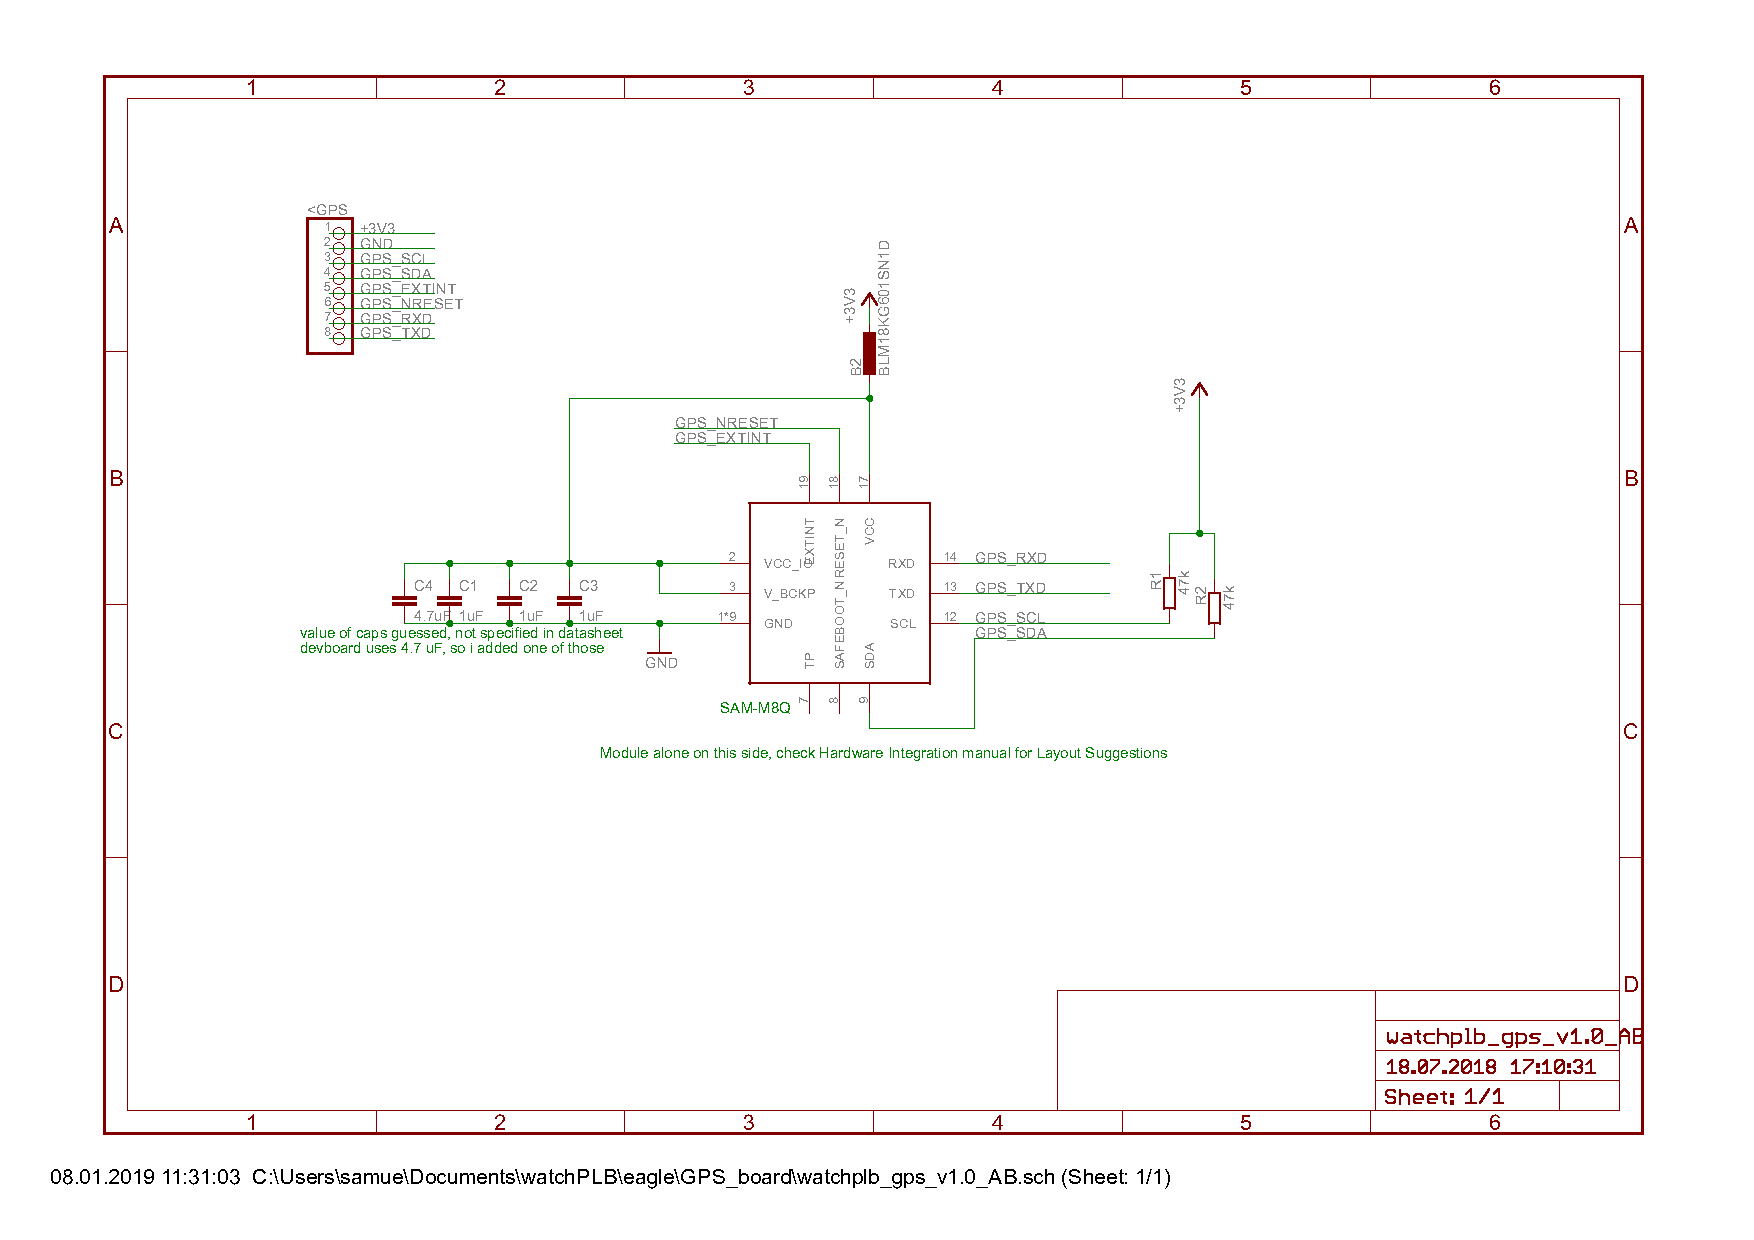
\includegraphics[page=1, angle=90, width=\linewidth]{../eagle/GPS_board/watchplb_gps_v1_0_AB.pdf}
\caption{GPS-Modul}
\end{figure}




\end{document}